\documentclass[11pt]{article}
\usepackage{times}
\usepackage{amsmath,amsthm,amssymb,setspace,enumitem,epsfig,titlesec,verbatim,color,array,eurosym,multirow}
\usepackage[sort&compress]{natbib}
\usepackage[footnotesize,bf]{caption}
\usepackage[margin=2.5cm, includefoot, footskip=30pt]{geometry}
\usepackage{standalone}
\usepackage{tikz}
\usepackage{subcaption}
\usepackage{hyperref}
\usepackage{tabularx}
\usepackage{booktabs}
\usepackage[ruled,vlined]{algorithm2e}
\smallskip % Erlaubt kleine Abstaende zwischen Paragraphen, falls es dem Seitenlayout hilft
\renewcommand{\baselinestretch}{1.3}
\newcommand{\R}{\mathbb{R}}

\definecolor{darkblue}{rgb}{0,0,.8}
\definecolor{darkgreen}{rgb}{0,0.5,0.1}
\newcommand{\matlabfunc}[1]{\textcolor{darkblue}{#1}}
\newcommand{\matlabcomment}[1]{\textcolor{darkgreen}{#1}}
\newcommand{\christian}[1]{\textcolor{blue}{\textbf{CH}: #1}}
\newcommand{\alex}[1]{\textcolor{red}{\textbf{AL}: #1}}

%% Adding shortcut commands to refer to our figures %%
\newcommand{\FigEvoProc}{{\bf Fig.~1}}
\newcommand{\FigInvAnalysis}{{\bf Fig.~2}}
\newcommand{\FigResultsOverPara}{{\bf Fig.~3}}


\titleformat{\section}{\sffamily \fontsize{12}{14}\bfseries}{\thesection}{1em}{}
\titleformat{\subsection}{\sffamily \fontsize{11.5}{11.5}\bfseries}{\thesubsection}{1em}{}

\usepackage{tikz}
\usetikzlibrary{arrows}

\tikzset{
  treenode/.style = {align=center, inner sep=0pt, text centered,
    font=\sffamily},
  arn_n/.style = {treenode, circle, white, font=\sffamily\bfseries, draw=black, inner sep=-6pt,
    fill=black, text width=1.5em},% arbre rouge noir, noeud noir
  arn_r/.style = {treenode, circle, red, 
    text width=1.5em, very thick, inner sep=4pt},% arbre rouge noir, noeud rouge
  arn_x/.style = {treenode, rectangle, draw=black,
    minimum width=0.5em, minimum height=0.5em}% arbre rouge noir, nil
}

\newtheoremstyle{plainCl1}% name
{9pt}%      Space above, empty = 'usual value'
{9pt}%      Space below
{\it}% 	   Body font
{}%         Indent amount (empty = no indent, \parindent = para indent)
{\bfseries}% Thm head font
{.}%        Punctuation after thm head
{0.2cm}% Space after thm head: \newline = linebreak
{}%         Thm head spec

\newtheoremstyle{plainCl2}% name
{9pt}%      Space above, empty = 'usual value'
{9pt}%      Space below
{\it}% 	   Body font
{}%         Indent amount (empty = no indent, \parindent = para indent)
{\bfseries}% Thm head font
{$'$.}%        Punctuation after thm head
{0.2cm}% Space after thm head: \newline = linebreak
{}%         Thm head spec

\newcommand{\splitatcommas}[1]{%
  \begingroup
  \begingroup\lccode`~=`, \lowercase{\endgroup
    \edef~{\mathchar\the\mathcode`, \penalty0 \noexpand\hspace{0pt plus 1em}}%
  }\mathcode`,="8000 #1%
  \endgroup
}

\theoremstyle{plainCl1}
\newtheorem{Claim}{Claim}
\newtheorem{Thm}{Theorem}
\newtheorem{Prop}{Proposition}
\newtheorem*{Lem}{Lemma}
\newtheorem{Cor}{Corollary}
\newtheorem*{Def}{Definition}

\theoremstyle{plainCl2}
\newtheorem{Claim2}{Claim}

\title{
\bf  \sffamily \LARGE Evolution of cooperation among individuals with limited payoff memory\\}
\date{}
\author{Christian Hilbe, Nikoleta E. Glynatsi, Alex McAvoy}

\begin{document}
\maketitle

\begin{abstract}
Repeated games have been the centerpiece when studying the evolution of human
cooperation. Most of the existing models work with idealized assumptions.
Individuals are assumed to interact with a representative sample of the
population, and they remember all interactions they participate in. In real
life, however, individuals do not always remember all interactions they had with
everyone in their population. Instead, they rather recall the last interaction
they had.

In this work we explore the effect on the evolution of cooperation if
individuals only remember a minimum of social information. We present results
for a series of simulations were we vary the benefit of cooperation and the
strength of selection. We present results for the most commonly used classes of
social dilemmas, and we show that even though cooperation can evolve when
individuals only use a minimum of information, the evolving cooperation rates
are typically lower than in the classical scenario.
\end{abstract}

\section{Introduction}

One of the most important applications of evolutionary game theory is the
evolution of cooperation. Why is it that some individuals choose to help others,
increasing their payoff, at the expense of decreasing one’s own? In evolutionary
game theory individuals are not required to be rational, instead they adapt
strategies based on mutation and exploration. Strategies are more likely to
spread if they have a high fitness either because the individuals who adopt them
have more offspring, or because they are imitated more often~\cite{Wu2015}. The
fitness of a strategy is not constant but depends on the composition of the
population. Individuals interact based on their strategies with other members of
the population and the payoffs they yield are translated into fitness.

It is commonly assumed that individuals compute their fitness after interacting
with a representative sample of the population, and remembering all the
interactions they participated in~\cite{Nowak2006}. Thus, they imply that
individuals have a perfect memory. However, when modelling how individuals make
decisions in each turn they are assumed to have very limited memory. To be
precise, most of the works in the literature focus on naive subjects who can
only choose from a restricted set of strategies~\cite{Nowak1992tit}, or who do
not remember anything beyond the outcome of the very last round~\cite{Baek2016}.
Note that there are a few notable exceptions~\cite{Hauert1997, Stewart2016}.
The perfect memory assumption is not only unrealistic but it also creates
this curious inconsistency.

This has led us to question the robustness of our understanding of cooperation.
In this work we explore whether cooperation can evolve if individuals compute
their fitness based on a minimum of social information. Though we are not the
first to question the assumptions of estimating fitness~\cite{Roca2006}, we are
the first to explore the effect of payoff memory. %ToDo add more information 

We first consider two extreme scenarios, the classical scenario of the expected
payoffs and the alternative scenario where individuals update their strategies
only based on the very last payoff they obtained. We observe that individuals
with limited memory tend to adopt less generous strategies and they achieve less
cooperation than in the classical scenario. We obtain similar results when we
consider that individuals update their strategies based on more social
information. More specifically, up to the last two payoffs they obtained when
interacting with up to two different members of the population.

The remainder of the paper is organized as follows. In
section~\ref{section:model} we describe the model. In
section~\ref{section:results} we present the results of the simulations, and
in section~\ref{section:conclusions} we outline the main conclusions.

\section{Model Setup}\label{section:model}

We consider a population of \(N\) players~\footnote{The terms ``player'' and
``individual'' are used interchangeably here.} where \(N\) is even and mutations
are sufficiently rare. Therefor, at any point in time there are at most two
different strategies present in the population; a \textit{resident} strategy and
a \textit{mutant} strategy. To describe how strategies spread we use a pairwise
comparison process~\cite{Traulsen2006}.
Each step of the evolutionary process consists of two
stages, a game stage and an updating stage.

In the game stage each individual is randomly matched with some other individual
in the population. They engage in a match where each subsequent turn
occurs with a fixed probability $\delta$. At each turn players can choose to
either cooperate (\(C\)) or to defect (\(D\)), and the payoffs of the turn
depend on both their decisions. If both players cooperate they receive the
reward payoff \(R\), whereas if both defect they receive the punishment payoff
\(P\). If one cooperates but the other defects, the defector receives the
temptation \(T\) payoff, whereas the cooperator receives the sucker's
payoff \(S\). We denote the feasible payoff of each turn as \(\mathcal{U} =
\{R, S, T, P\}\).
We assume that individuals use \textit{reactive strategies} to make
decisions in each turn. Reactive strategies are a set of memory-one strategies
that only take into account the previous action of the opponent. They can be
written explicitly as a vector \(\in \R_{3}\), more specifically, a reactive
strategy \(s\) is given by \(s=(y, p, q)\) where \(y\) is the probability that
the strategy opens with a cooperation and \(p, q\) are the probabilities that
the strategy cooperates given that the opponent cooperated and defected
equivalently.

In the updating stage, two players are randomly drawn from the population, a
`learner' and a `role model'. Given that the learner's payoff $u_L\!\in\!
\mathcal{U}$ and that the role model's payoff $u_{RL}\!\in\! \mathcal{U}$.
The learner adopts the role model's strategy based on the Fermi
distribution function,

\begin{equation} \label{Eq:rho}
  \rho(u_{L}, u_{RM}) = \frac{1}{1\!+\! \exp^{\!-\!\beta (u_{RM}\!-\!u_{L})}}.
\end{equation}

where $\beta\!\ge\!0$ is the intensity of selection. The updating payoffs of the
learner and the role model are conventionally correspond to their expected
payoffs. The expected payoff of a strategy is the mean payoff of the strategy of
engaging in repeated games with all other members of the population. The expected payoffs
assume perfect memory. In this work we define a new a set of updating
payoffs. We reefer to these as the limited memory payoffs, and we compare them
to the classical scenario.

The evolutionary step is repeated until either the mutant strategy goes
extinct, or until it fixes in the population. If the mutant fixes in the
population then the mutant strategy becomes the new resident strategy. After
either outcome we introduce a new mutant strategy uniformly chosen from all
reactive strategies at random, and we set the number of mutants to $1$. This
process of mutation and fixation/extinction is then iterated many times.
More details on our methodology are found in Appendix~\ref{appendix:methods}.

In order to account for the effect of the updating payoffs approaches, we
explore the cooperation rate within the resident population over multiple
generations. In the next section we present a series of simulation results.
To account for the various types of social behaviour we also present
results on multiple social dilemmas.


\section{Results}\label{section:results}
\subsection{Updating payoffs based on the last round with another member of the population}\label{section:donation}

In this section we explore the case where the updating payoffs are based on the
last round payoff achieved against another member of the population and we compare
this to the classical scenario of the expected payoffs. We assume that each pair
of players interacts in a donation game. The donation game is a special case of
the prisoner's dilemma. Each player can choose to cooperate by providing a
benefit \(b\) to the other player at their cost \(c\), with \(0 < c < b\).
Thus, the feasible payoffs in each round are \(T=b, R=b-c, S=-c, P=0\).

Figure~\ref{fig:expected_and_stochastic_for_donation} shows simulations results
for the described process of section~\ref{section:model}.
Figure~\ref{fig:expected_and_stochastic_for_donation} depicts the evolving
conditional cooperation probabilities $p$ and $q$. The discount factor~$\delta$
is comparably high, thus we do not report the opening move \(y\) as it
is a transient effect. The left panels correspond to the
standard scenario considered in the literature, it considers players who use
expected payoffs to update their strategies. The right panel shows the scenario
considered herein, in which players update their strategies based on their last
round’s payoff. The top panels assume a benefit \(b\) of 3 whereas the bottom
assume a benefit of 10.

The figure suggests that when updating is based on expected payoffs players
tend to be more generous and more cooperative. The $q$-values of the resident
strategies are on average higher in the case of the expected payoffs. The
players will occasionally forgive a defection more often if their fitness
depends on interacting with every member of the population. On the other hand,
when social interactions are limited they are less forgiving. The average
cooperation rate for each simulation is calculated as the average
cooperation rate within the resident population. In the case of the expected
payoffs, regardless the value of benefit, the average cooperation rate is
strictly higher than that of the last round payoffs. The difference based on the
two methods is statistically significant, and in the case of $b=10$ the
average cooperation of resident strategies drops from 97\% to 57\%.

\begin{figure}[!htbp]
    \centering
    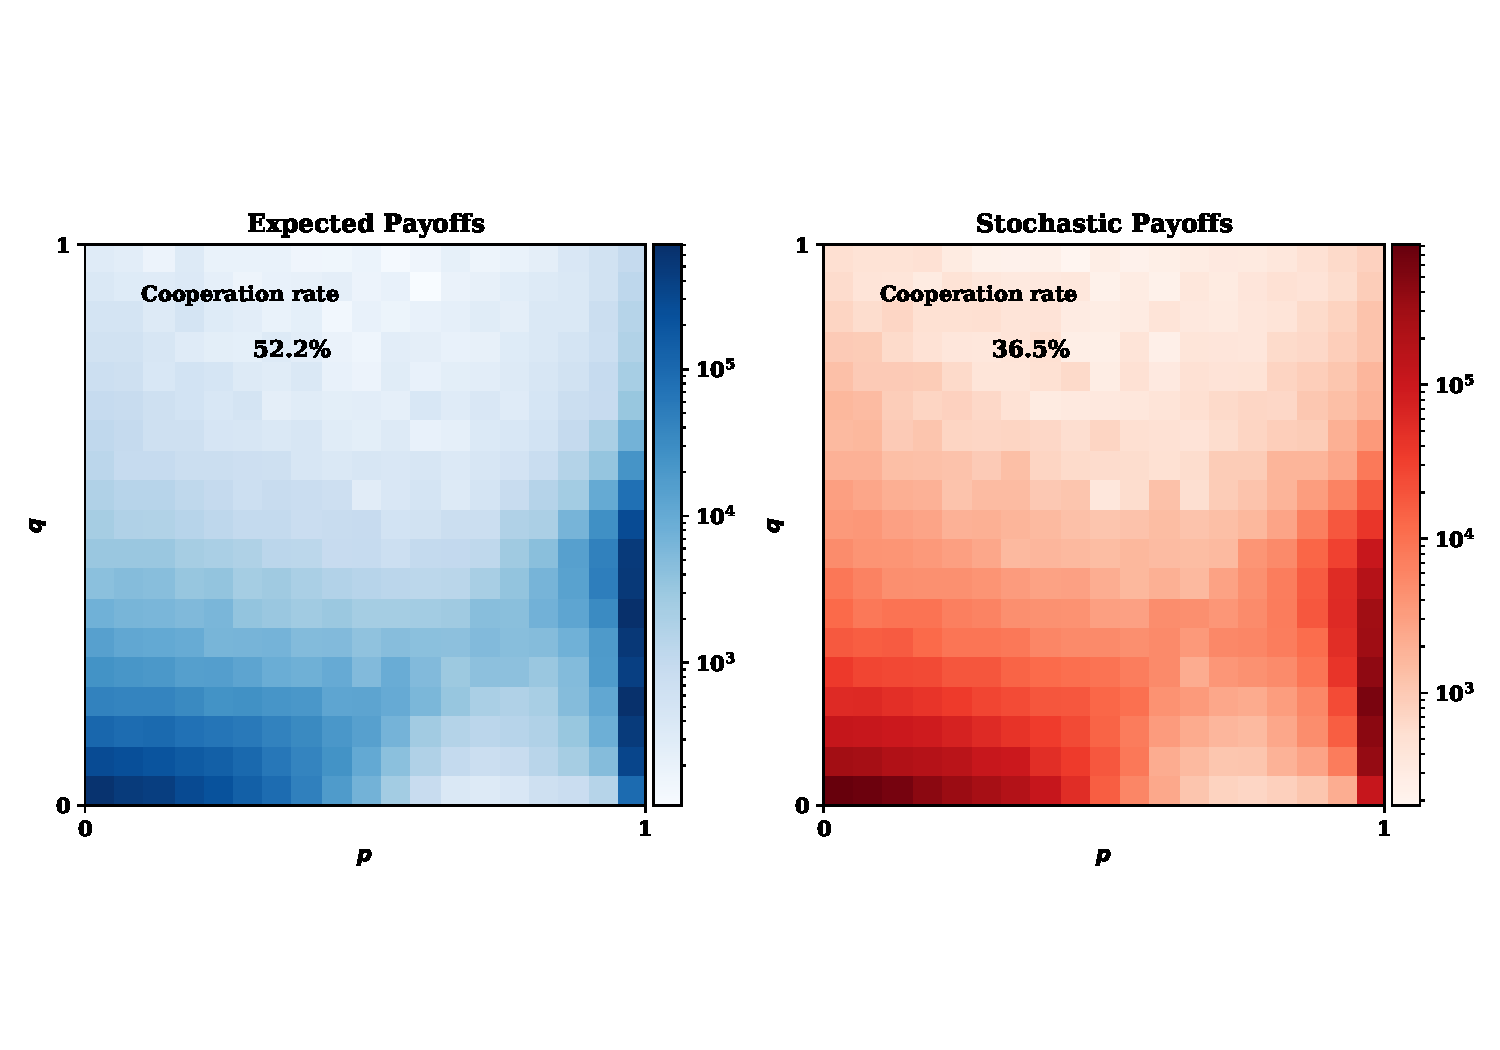
\includegraphics[width=.70\textwidth]{static/expected_and_stochastic_for_donation_game.pdf}\vspace{-3cm}
    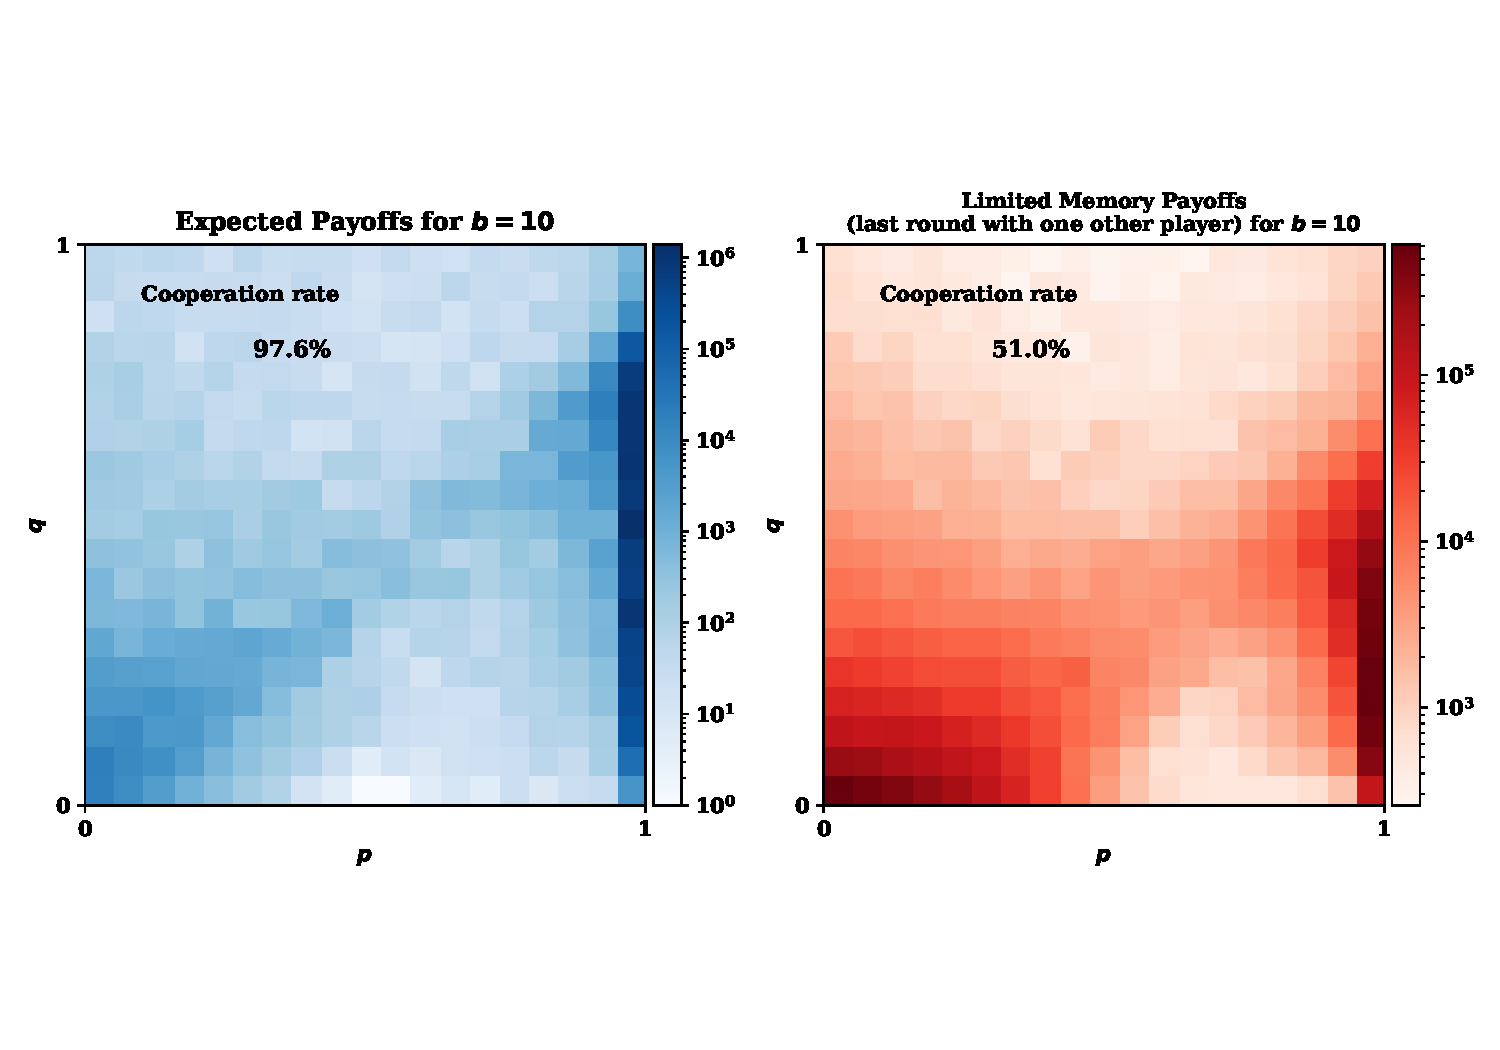
\includegraphics[width=.70\textwidth]{static/expected_and_stochastic_for_donation_game_b_10.pdf}
    \caption{{\bf Evolutionary dynamics under expected payoffs and last round with one interaction payoffs.} 
    We have run two simulations of the evolutionary process described in
    section~\ref{section:model} for $T\!=\!10^7$ time steps. For each time step,
    we have recorded the current resident population ($y,p,q$). Since simulations
    are run for a relatively high continuation probability of $\delta\!=\!0.999$, we
    do not report the players' initial cooperation probability $y$. The graphs show
    how often the resident population chooses each combination ($p,q$) of
    conditional cooperation probabilities in the subsequent rounds. ({\bf A}) If
    players update based on their expected payoffs, the resident population
    typically applies a strategy for which $p\!\approx\!1$ and
    $q\!\le\!1\!-\!c/b\!=\!0.9$. ({\bf B})
    When players update their strategies based on their realized payoffs in the last
    round, there are two different predominant behaviors. The resident population
    either consists of defectors (with $p\!\approx\!q\!\approx\!0$) or of
    conditional cooperators. In the latter case, the maximum level of $q$ consistent
    with stable cooperation is somewhat smaller compared to the expected-payoff
    setting, $q\!<\!0.5$. The cooperation rate within the resident population
    (averaged over all games and over all time steps) is close to 100\%. Parameters:
    $N\!=\!100$, $c\!=\!1$, $\beta\!=\!1$, $\delta\!=\!0.999$.}
    \label{fig:expected_and_stochastic_for_donation}
\end{figure}

We further explore the effect of benefit in
Figure~\ref{fig:cooperation_rate_over_benefit}. The figure suggests that
expected payoffs always yield a higher cooperation rate. In the case of expected
payoffs we observe that the cooperation rate increases as the value of the
benefit gets higher. In comparison for the limited memory payoffs, the
cooperation rate remains unchanged at approximately 50\% once \(b=5\).

\begin{figure}[!htbp]
  \centering
  \begin{subfigure}{.5\textwidth}
    \centering
    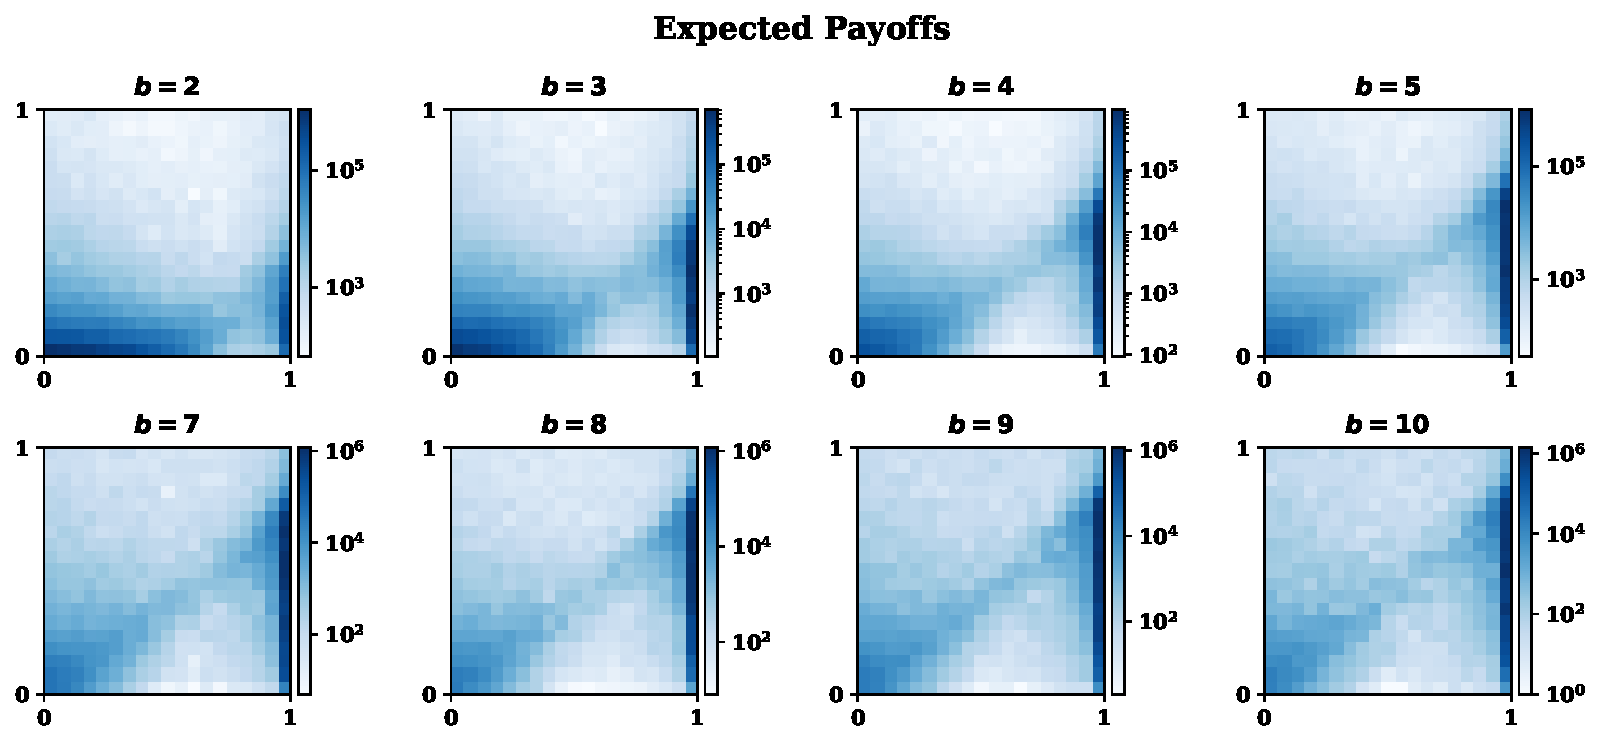
\includegraphics[width=.8\textwidth]{static/expected_for_beta.pdf}
    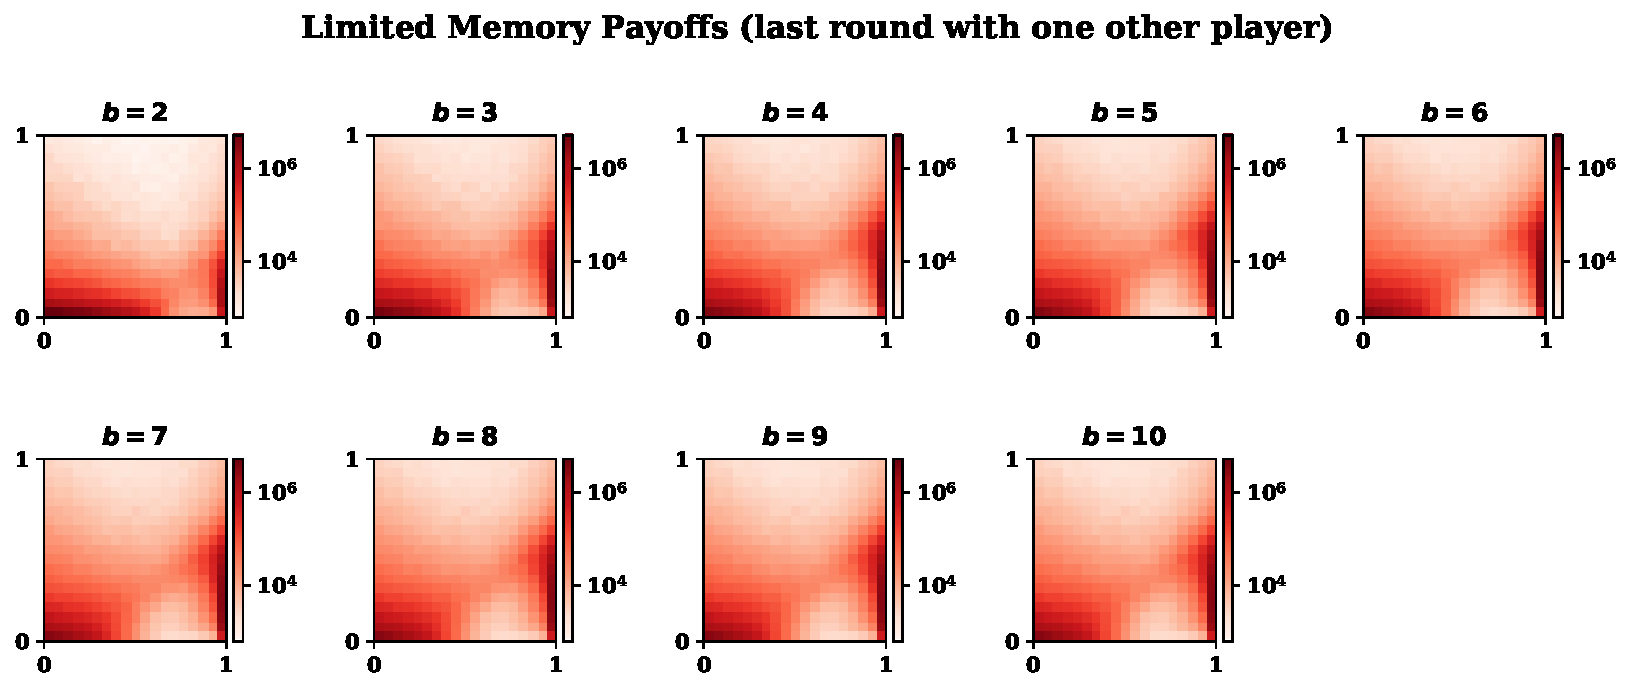
\includegraphics[width=.8\textwidth]{static/stochastic_for_beta.pdf}
  \end{subfigure}%
  \begin{subfigure}{.5\textwidth}
    \centering
    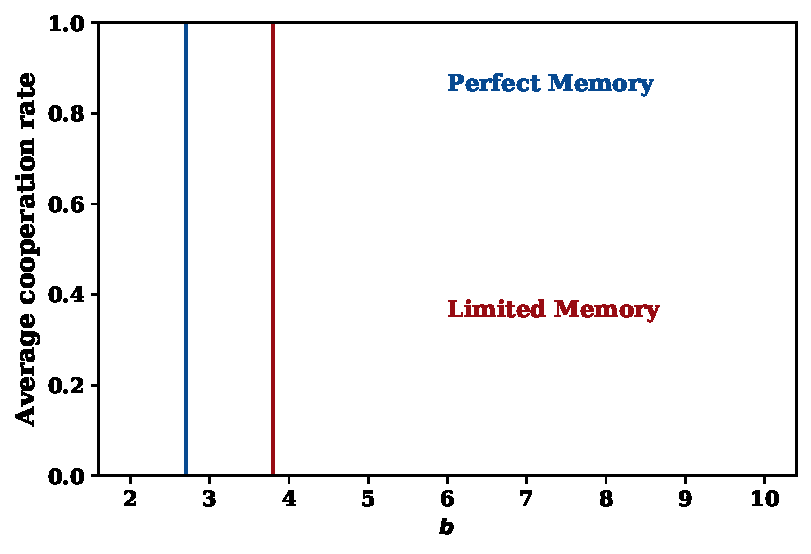
\includegraphics[width=.8\textwidth]{static/cooperation_rate_over_b.pdf}
  \end{subfigure}
  \caption{{\bf The evolution of cooperation for different benefit values.} 
  We vary the benefit of defection $b$. In all cases, expected payoffs appear to
  overestimate the average cooperation rate the population achieves. ({\bf A})
  the probabilities \(p, q\) for resident population over \(10^7\) time steps
  for each benefit value. ({\bf B}) The cooperation rate within the resident population
  (averaged over all games and over all time steps) over the benefit.
  Unless
  explicitly varied, the parameters of the simulation are $N\!=\!100$,
  $c\!=\!1$, $\beta\!=\!1$, $\delta\!=\!0.99$. Simulations are run
  for $T\!=\!5\times 10^7$ time steps for each parameter
  combination.}\label{fig:cooperation_rate_over_benefit}
\end{figure}

We also investigate the effect of the strength of selection $\beta$.
Figure~\ref{fig:cooperation_rate_over_betas} illustrates results for various
runs of the evolutionary process. For weak selection, \(\beta < 1\), we observe
that the two methods yield similar results, however, as \(\beta\) increases
there is variation in the evolving populations. In the case of expected payoffs
the resident populations become more cooperative as \(\beta\)
increases, whereas in the case of limited memory payoffs, the resident
populations become more defective.

\begin{figure}[!htbp]
  \centering
  \begin{subfigure}{.65\textwidth}
    \centering
    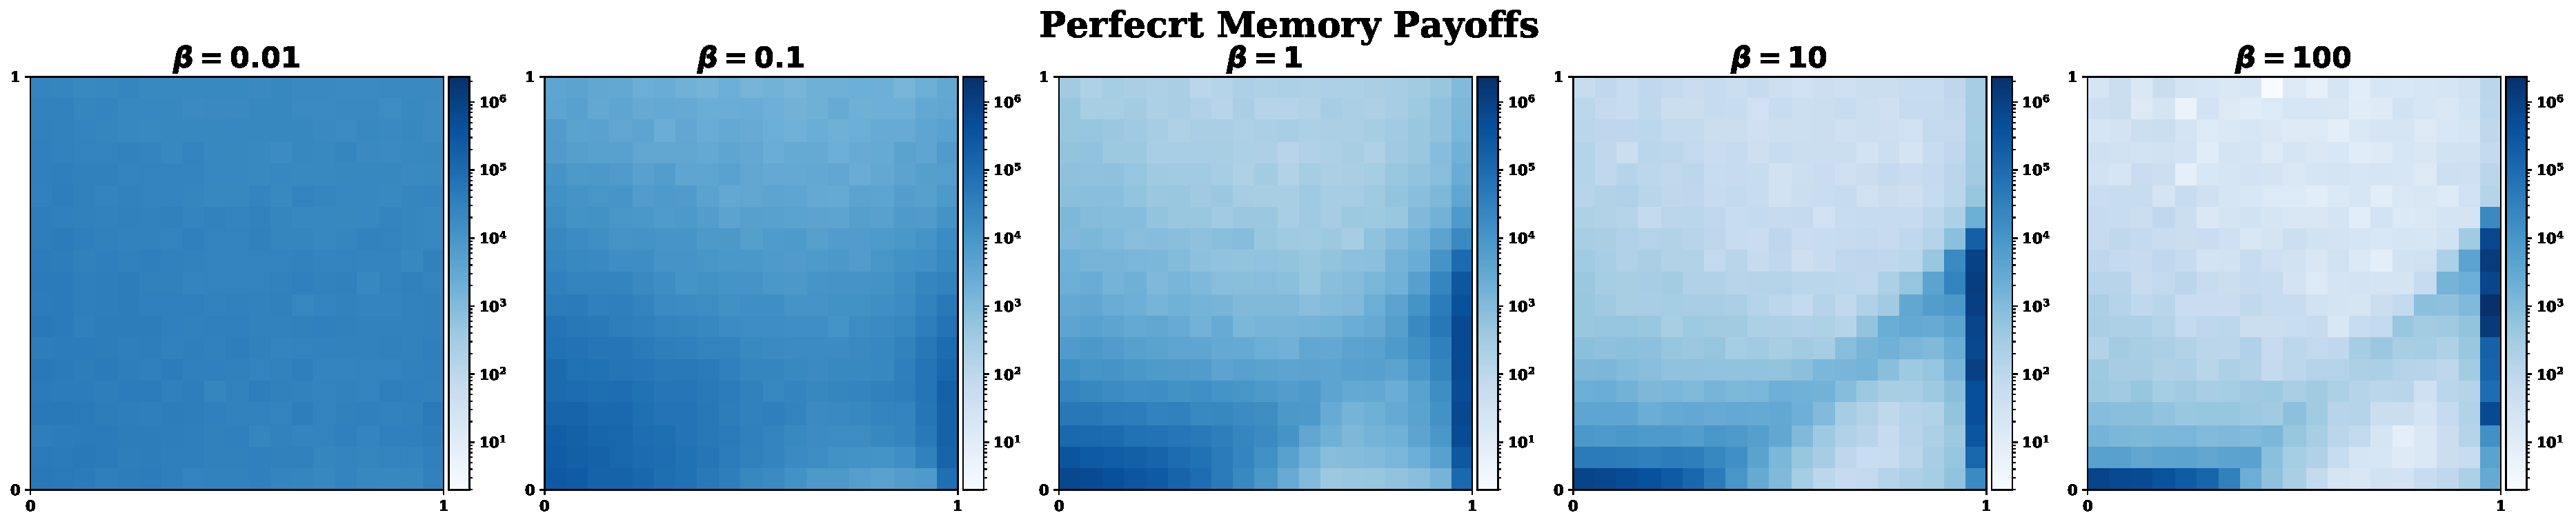
\includegraphics[width=.8\textwidth]{static/expected_for_selection_strenght.pdf}
    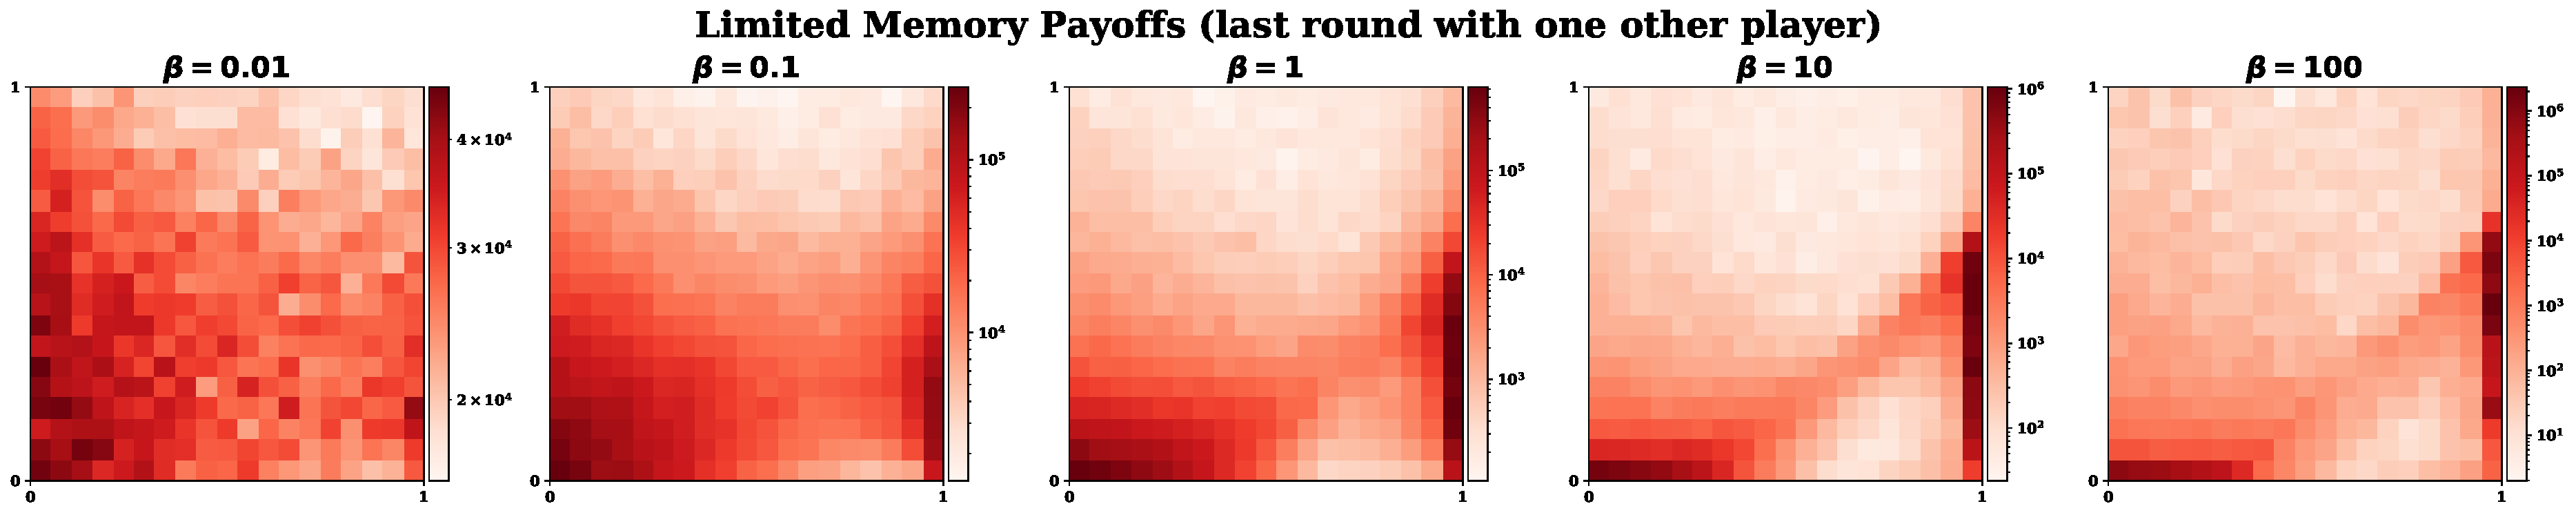
\includegraphics[width=.8\textwidth]{static/stochastic_for_selection_strenght.pdf}
  \end{subfigure}%
  \begin{subfigure}{.35\textwidth}
    \vspace{.3cm}
    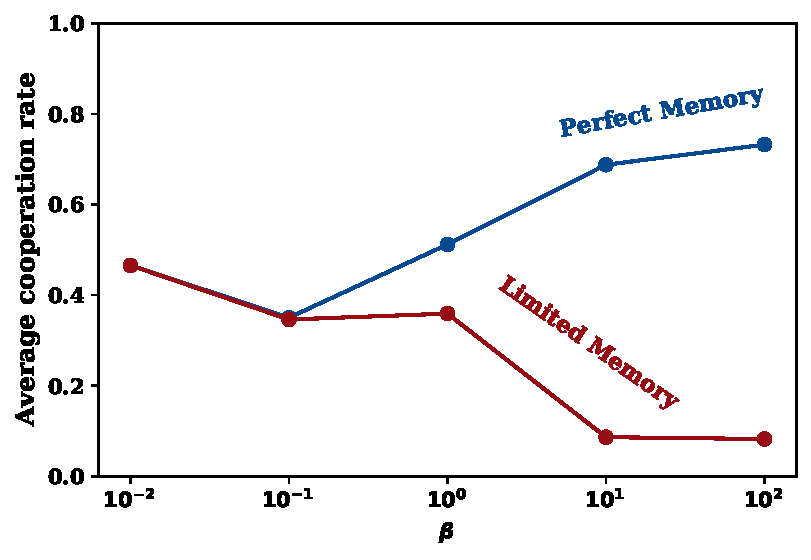
\includegraphics[width=.8\textwidth]{static/cooperation_rate_over_betas.pdf}
  \end{subfigure}
\caption{{\bf The evolution of cooperation for different selection strength values.}
We vary the selection strength $\beta$. In all cases, stochastic payoff
evaluation tends to reduce the evolving cooperation rates. ({\bf A}) the
probabilities \(p, q\) for resident population over \(10^7\) time steps for each
\(\beta\) value. ({\bf B}) The cooperation rate within the resident population
(averaged over all games and over all time steps) over \(\beta\).
Unless explicitly varied, the parameters of the simulation are $N\!=\!100$,
$b\!=\!3$, $c\!=\!1$, $\beta\!=\!1$, $\delta\!=\!0.99$. Simulations are run for
$T\!=\!5\times 10^7$ time steps for each parameter
combination.}\label{fig:cooperation_rate_over_betas}
\end{figure}

\subsection{Effect of updating payoffs in different social dilemmas}\label{section:2_by_2_games}

In the previous section we gained insights into the effects of the updating
payoffs, and into how parameters such as the benefit and the strength of
selection can intensify them. We investigated these effects by using the
donation game. In order to broaden our understanding of the updating payoffs on
different forms of possible human interactions we extend our approach to other
\(2 \times 2\) symmetric games. More specifically, we apply our analysis to four
different classes of games as given by Table~\ref{table:social_dilemmas}.

\begin{table}[!htbp]
  \begin{center}
    \resizebox{.4\textwidth}{!}{
    \renewcommand{\arraystretch}{1.5}
      \begin{tabular}{ccc}
  \toprule
  & \textbf{social dilemmas} & \textbf{preference ordering} \\
  \midrule
(i) & harmony  & \(R > T > S > P\) \\
(ii) & stag hunt  & \(R > T > P > S\) \\
(iii) & prisoner dilemma  & \(T > R > P > S\) \\
(iv) & snowdrift  & \(T > R > S > P\) \\
  \bottomrule
      \end{tabular}}
  \end{center}
\caption{\textbf{Social dilemmas and preference ordering}. The four classes of
social dilemmas we explore in this work.}
\label{table:social_dilemmas}
\end{table}

We compare the results of the evolutionary process described in
section~\ref{section:model} when the updating payoffs are based on the expected
payoffs, and on the last round payoffs for all the four possible classes of
games. The results of the simulations are given in
Figures~\ref{fig:expected_two_by_two} and~\ref{fig:last_round_two_by_two}
respectively.

In Figure~\ref{fig:expected_two_by_two} each sub figure represents a run of
evolutionary process for a different set of values for \(\mathcal{U}\). Without
loss of generality we set \(R=1\) and \(P=0\)~\cite{Martinez2012, Roca2009}, and
we vary the values of the temptation payoff \(T\) (across the \(x\)-axis) and of
the sucker's payoff \(S\) (across the \(y\)-axis). Starting at the upper left
corner and proceeding clockwise the quadrants correspond to the harmony, the
snowdrift, the prisoner's dilemma and the stag hunt games.

The harmony game represents are social situation without conflict. It is in the
best interest for both players to cooperate as \(R > T\) and \(S > P\).
Figure~\ref{fig:expected_two_by_two} confirms this. We observe that for most
harmony game runs the resident population overwhelmingly applies a strategy for
which \(p\) and \(p\) are \(\approx 1\). In the case of \(T = R = 1\) we observe
that the resident strategies become slightly less generous. Against a cooperating
strategy defecting and cooperation yield the same result. The lower \(q-\)values
could indicate that the resident strategy is less generous to defectors to avoid
being invaded.

The snowdrift game describes a situation similar to that of the prisoner's
dilemma. Cooperation results in a benefit to the opposing player but entailing a
cost to the cooperator. However, in the snowdrift game individuals obtain
immediate direct benefits from the cooperative acts which leads to \(S > P\). In
the snowdrift game more cooperation emerges compared to the prisoner's dilemma.
Defection is never a resident strategy and for the shame values of temptation
the overall \(q-values\) are higher. It can be seen that the \(p-values\) are
lower as individuals have free room to defect after receiving a cooperation.

The last class of games we present are for the stag hunt game. In the stag hunt
both players benefit for mutual cooperation and defection, however, \(R > P\)
and thus the resident strategies with the highest fitness are the cooperative
ones. The results for the stag hunt class are similar to those of the harmony
game.

\begin{figure}[!htbp]
  \centering
  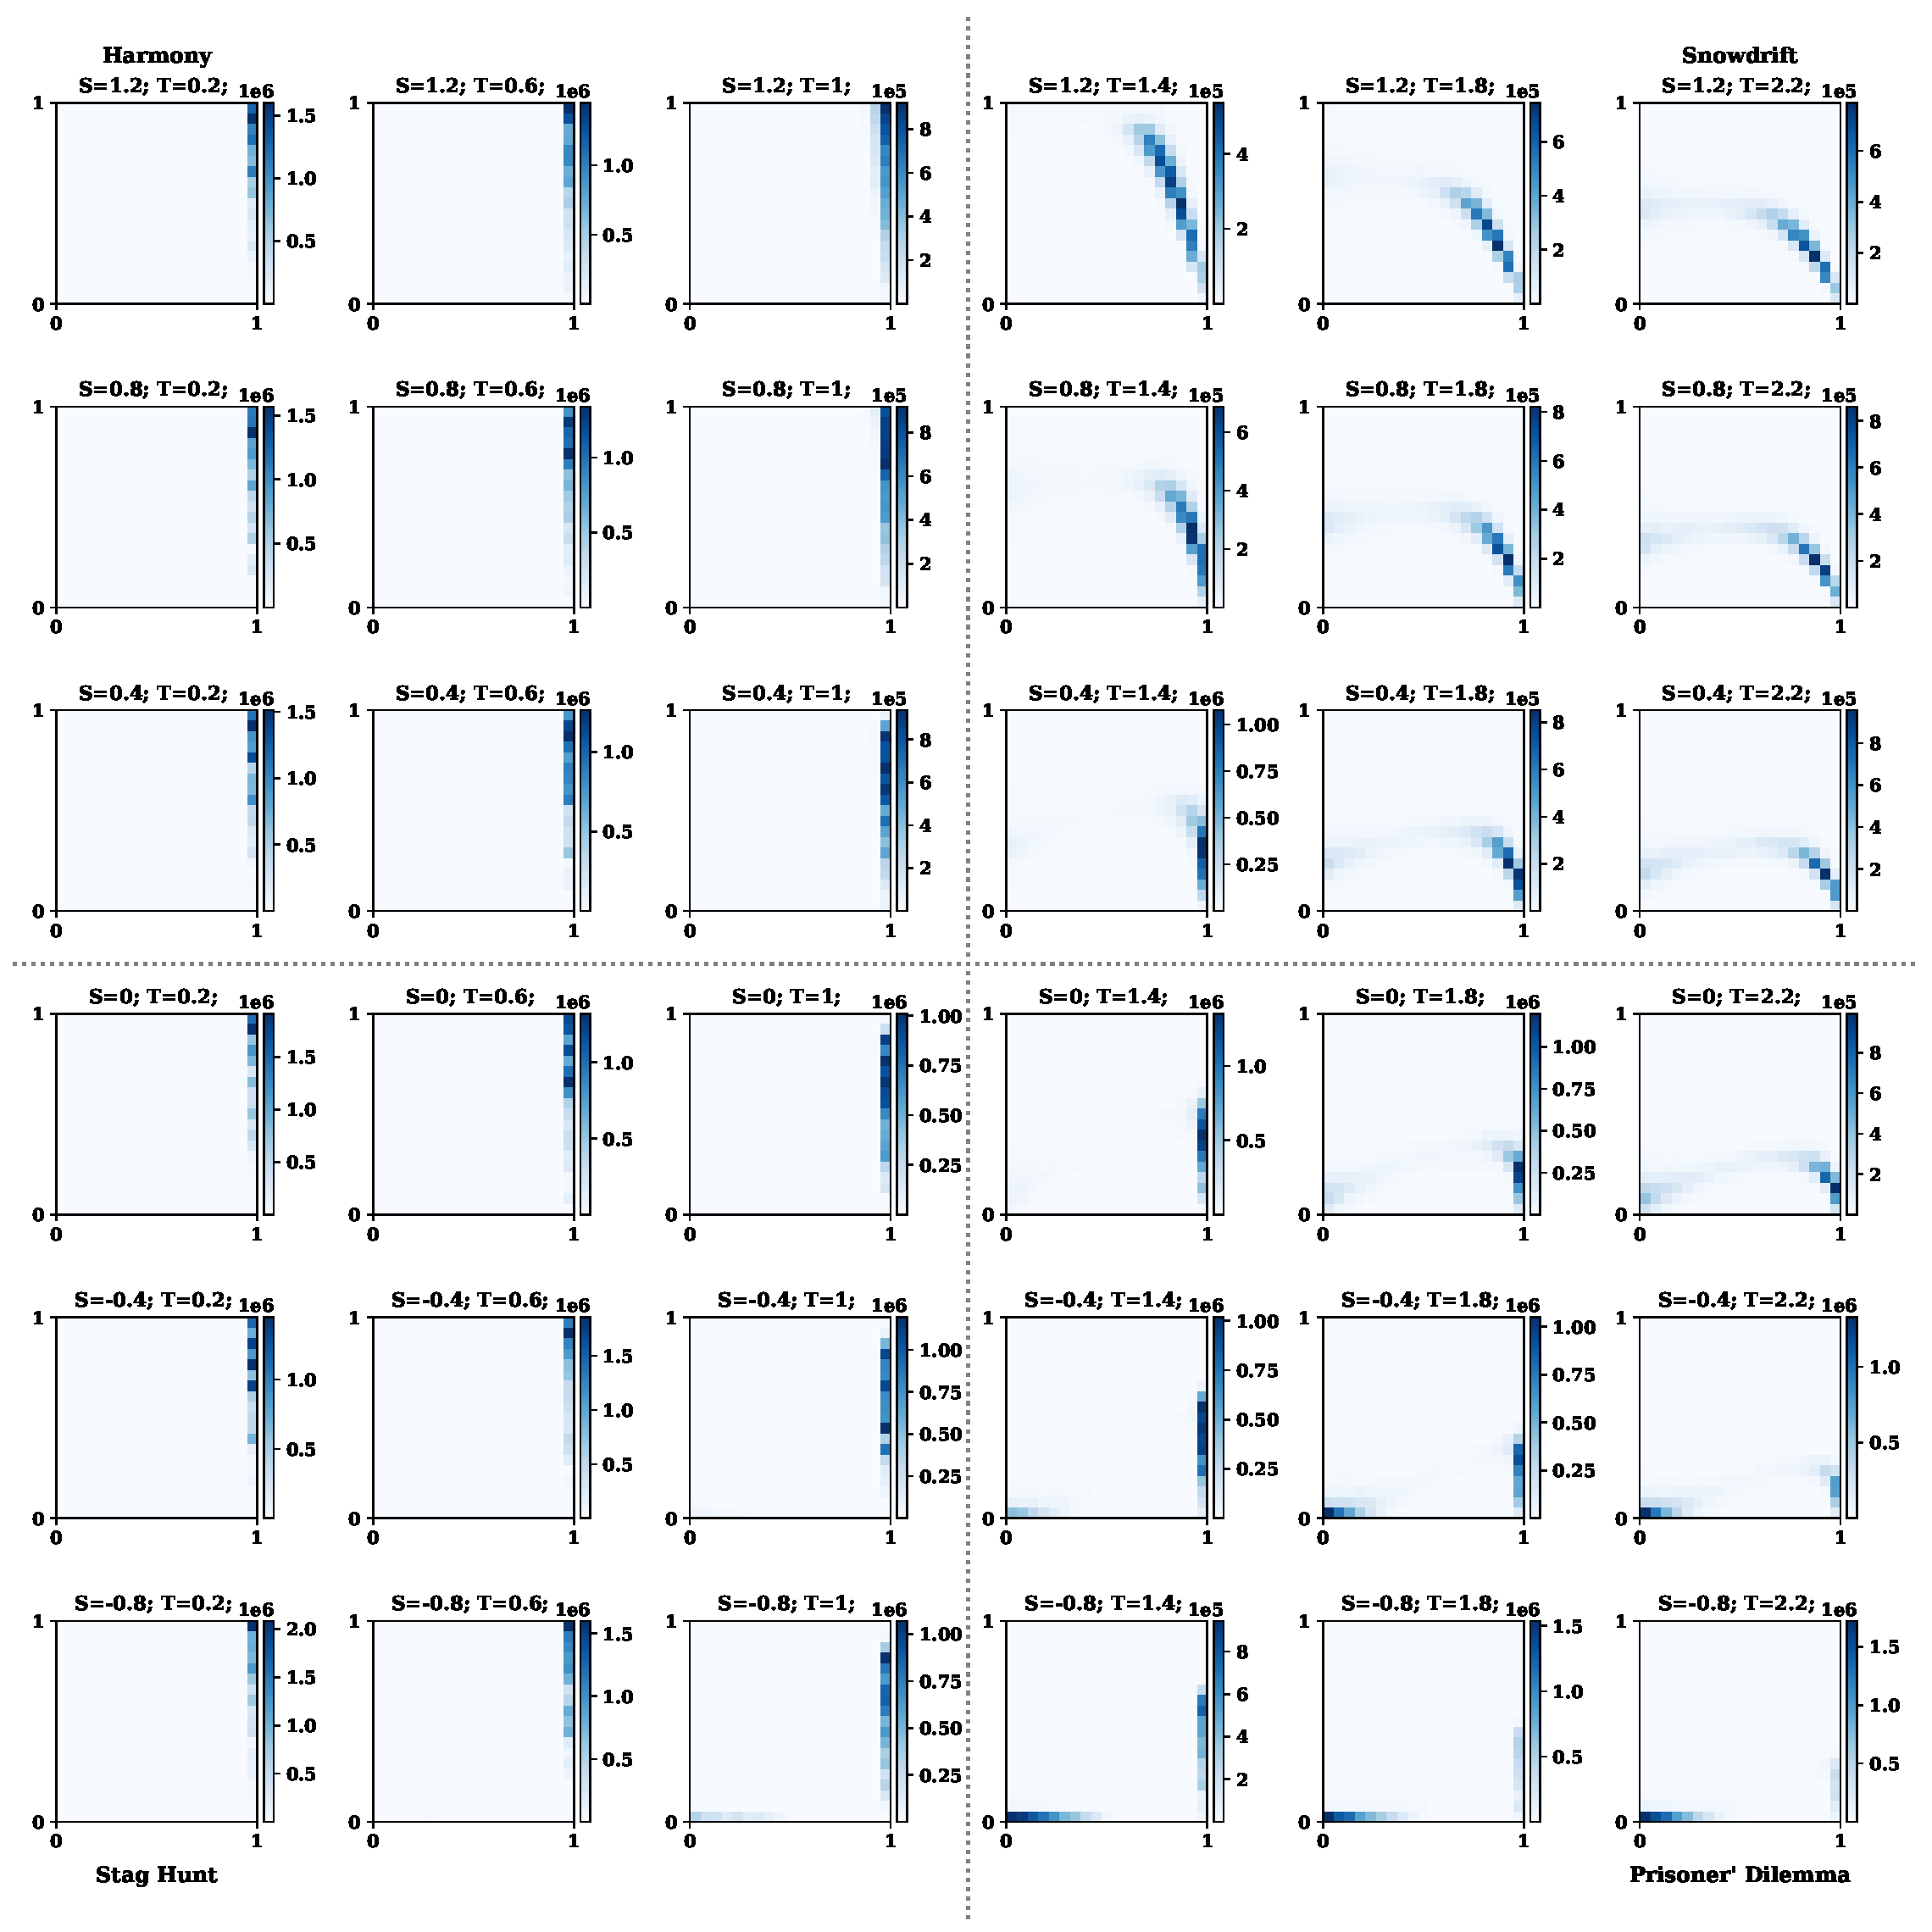
\includegraphics[width=\textwidth]{static/expected_two_by_two_games.pdf}
  \caption{{\bf Evolutionary dynamics under expected payoffs for various social dilemmas.} 
  We have run several simulations of the evolutionary process described in
  section~\ref{section:model} for $T\!=\!10^7$ time steps. The graphs show how
  often the resident population chooses each combination ($p,q$) of conditional
  cooperation probabilities in the subsequent rounds. We vary the temptation
  payoff \(T \in \{0.2, 0.6, 1, 1.4, 1.8, 2.2\}\)
  across the \(x\) axis, and  \(S \in \{1.2, 0.8, 0.4, 0, -0.4, -0.8\}\)
  across the \(y\) axis. Unless explicitly varied, the parameters of the simulation
  are $N\!=\!100$, $\beta\!=\!10$, $\delta\!=\!0.99$.}
  \label{fig:expected_two_by_two}
\end{figure}

The conclusions regarding the evolved behaviour for the various classes of
games remain the same when the last round payoffs are considered,
Figure~\ref{fig:last_round_two_by_two}. However, there is variation in these
populations. This variation as an effect affects the resident within cooperative
rates.


\begin{figure}[!htbp]
  \centering
  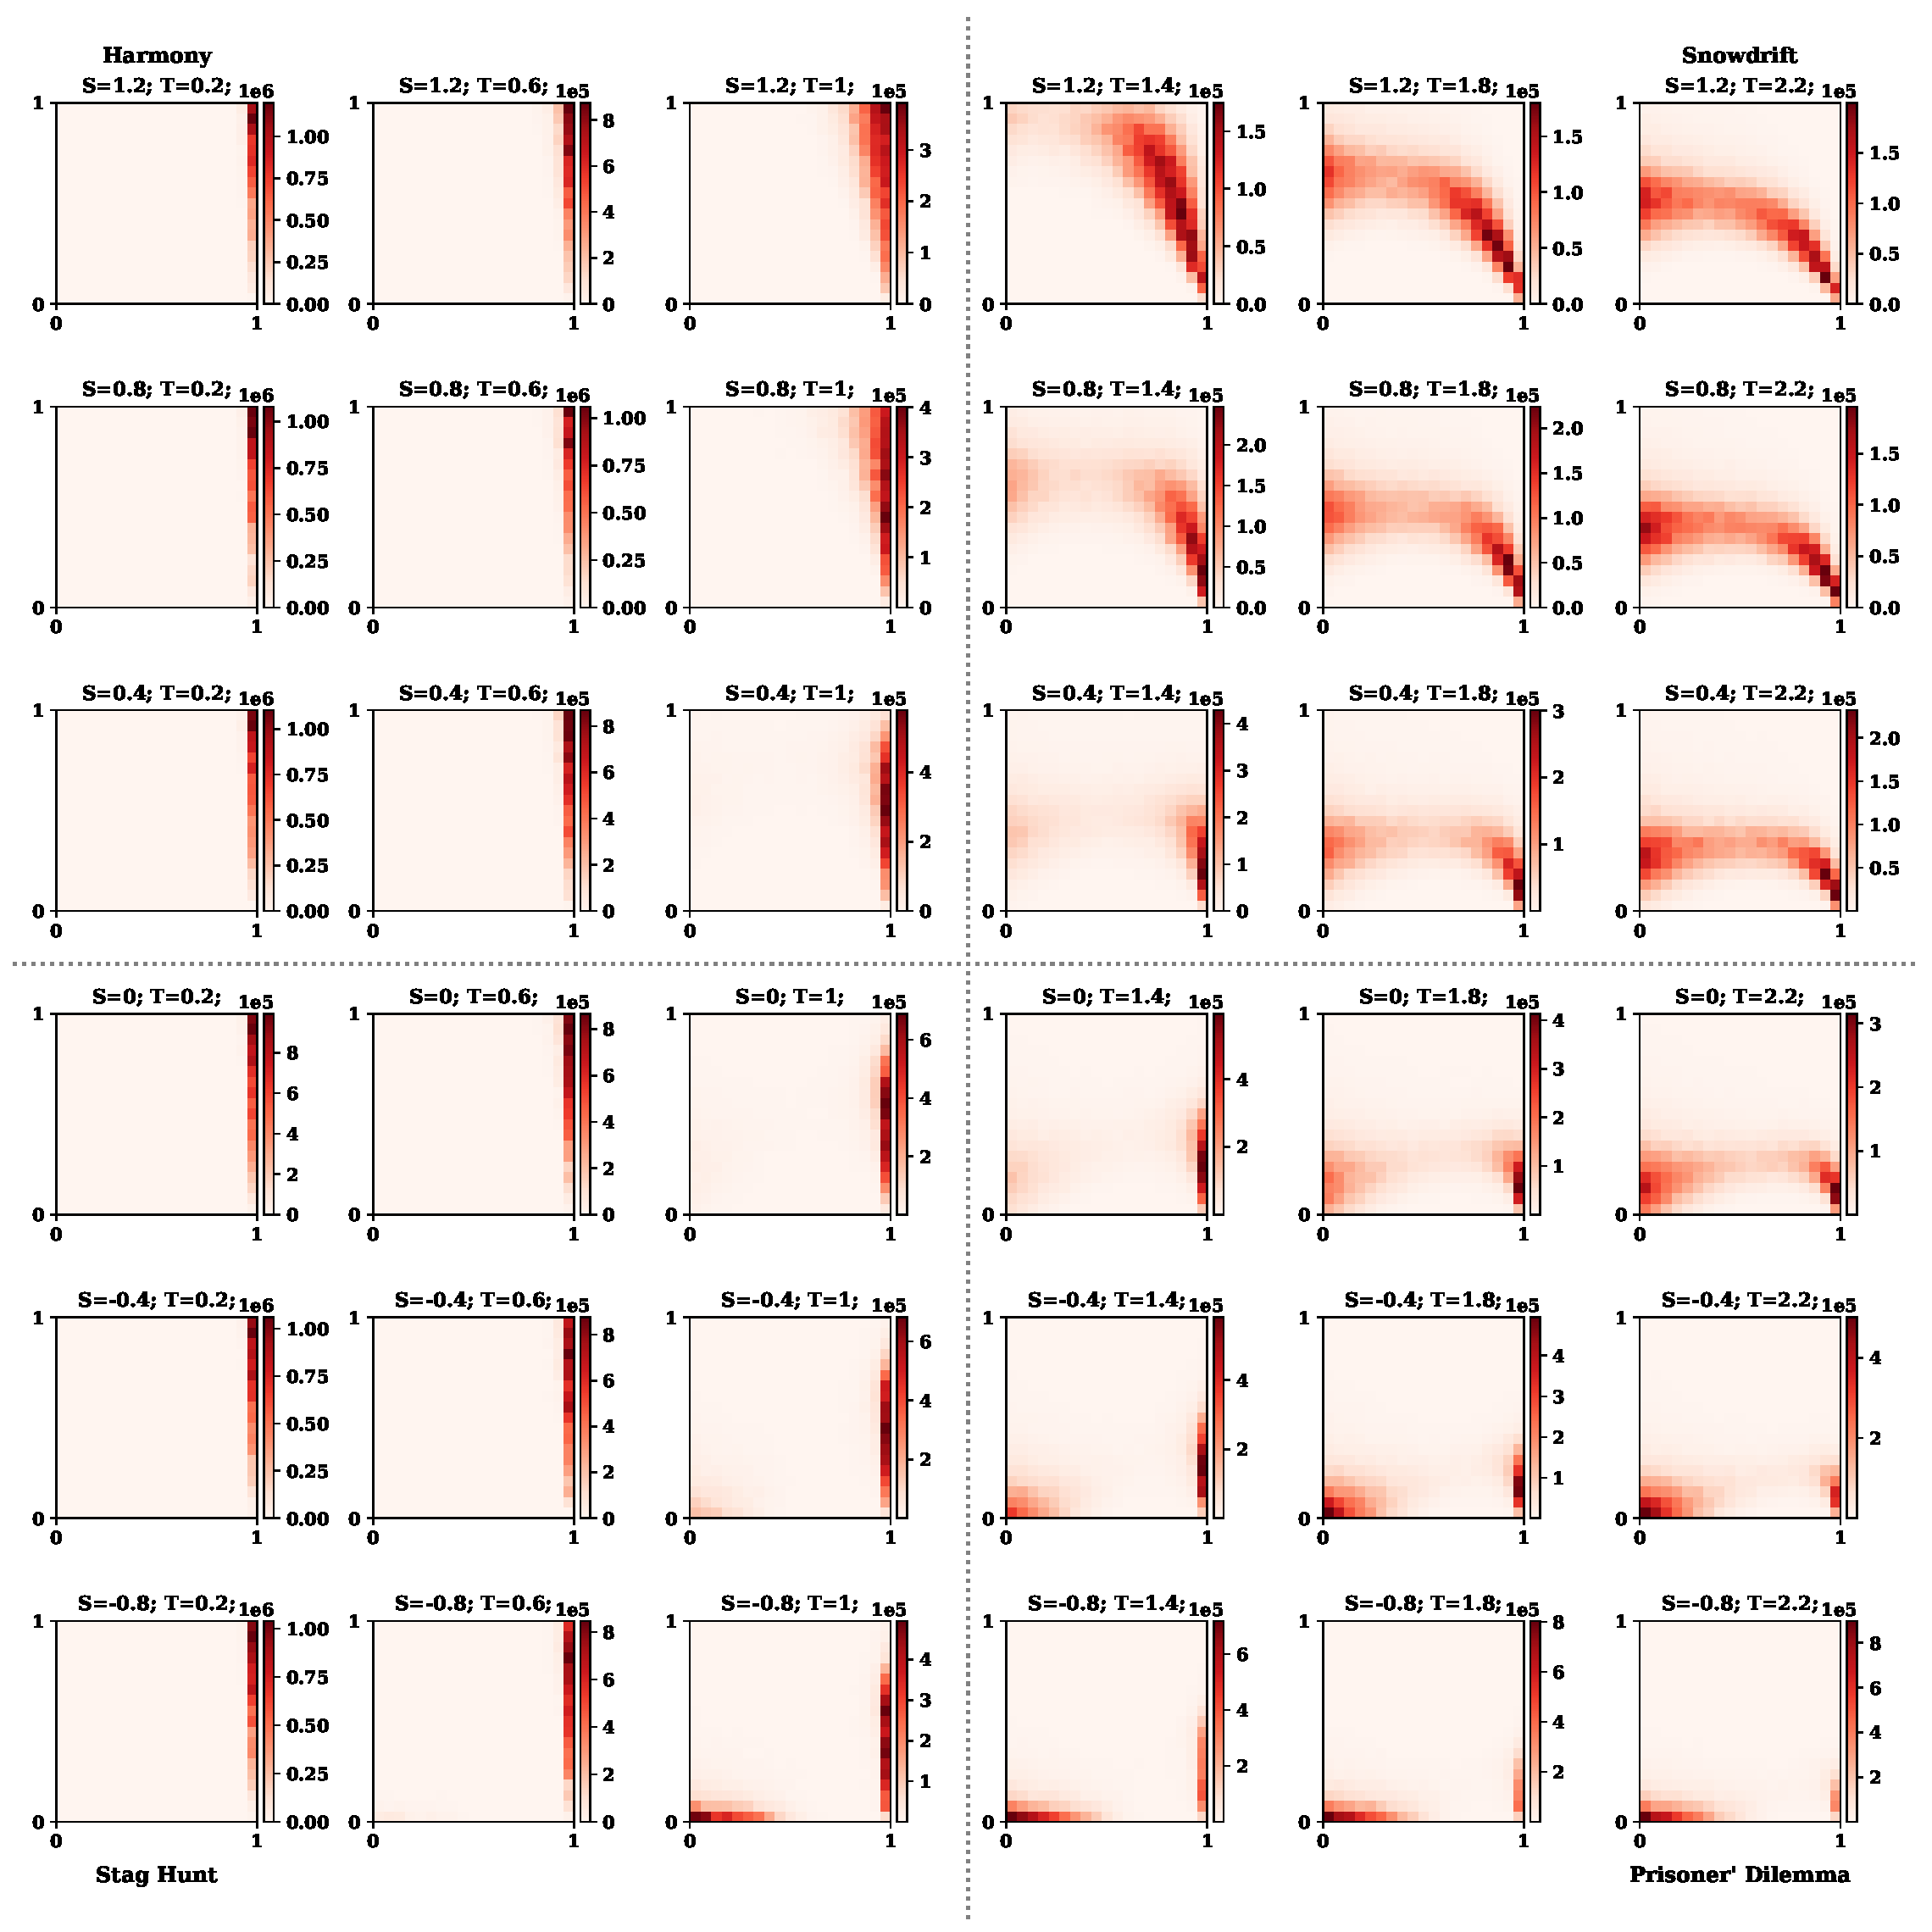
\includegraphics[width=\textwidth]{static/stochastic_two_by_two_games.pdf}
  \caption{{\bf Evolutionary dynamics under last round payoffs for various social dilemmas.} 
  We have run several simulations of the evolutionary process described in
  section~\ref{section:model} for $T\!=\!10^7$ time steps. The graphs show how
  often the resident population chooses each combination ($p,q$) of conditional
  cooperation probabilities in the subsequent rounds. We vary the temptation
  payoff \(T \in \{0.2, 0.6, 1, 1.4, 1.8, 2.2\}\)
  across the \(x\) axis, and \(S \in \{1.2, 0.8, 0.4, 0, -0.4, -0.8\}\)
  across the \(y\) axis. Unless explicitly varied, the parameters of the simulation
  are $N\!=\!100$, $\beta\!=\!10$, $\delta\!=\!0.99$.}
  \label{fig:last_round_two_by_two}
\end{figure}

The cooperation rates for each of the case of the social dilemmas we have used
are given in Figure~\ref{fig:cooperation_rates_two_by_two_part_one}. In the case
of the harmony game the differences are very small, even in the case of \(T=1\)
where the biggest difference occurs it still remain less than 10\%. In the case
of the stag hunt game the difference increases in the case of \(T=1\). The
biggest variation in the results are for the class of the prisoner's dilemma.
For values of \(S < -0.4\) the are significantly different, in the case of the
last round payoffs cooperation almost never is a valid option. Overall the last
round payoffs are less cooperative, supporting the results of the previous
section. There are only two cases which that is not true and both cases are in
the snowdrift class. For the values of \(T>1.8\) and \(S=0.4, 0.8\) cooperation
is estimated higher. In the last round payoffs a Tit For Tat like behaviour is
more robust that in the case of the expected payoffs.

\begin{figure}[!htbp]
  \centering
  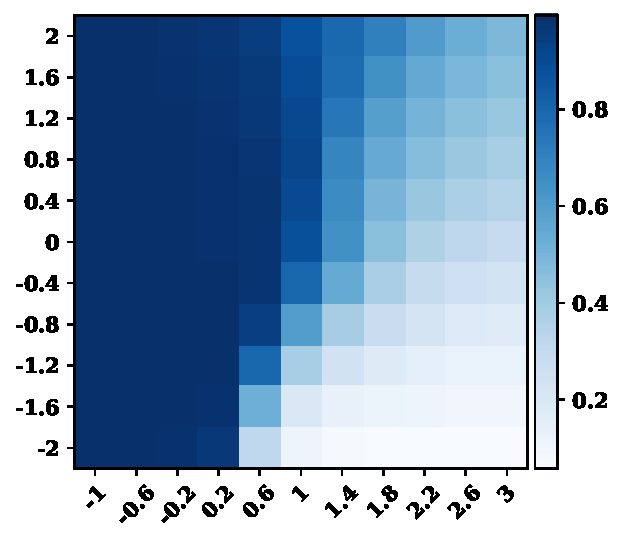
\includegraphics[width=.4\textwidth]{static/expected_two_by_two_games_cooperation.pdf}
  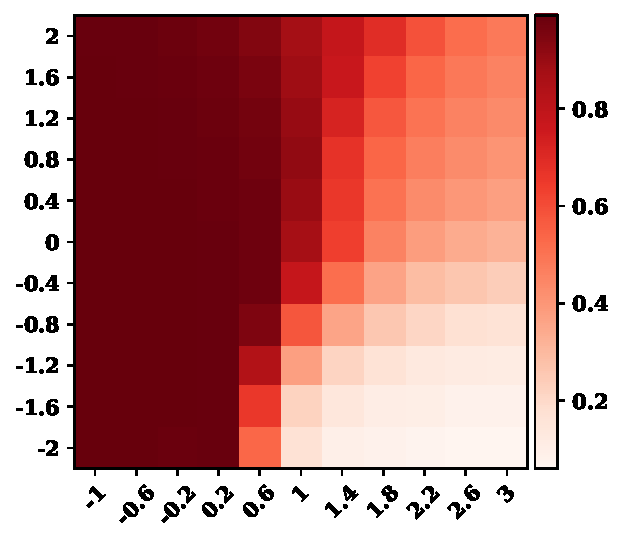
\includegraphics[width=.4\textwidth]{static/stochastic_two_by_two_games_cooperation.pdf}
  \caption{\textbf{Cooperation rates over various social dilemmas.} ({\bf A}) If
  players update based on their expected payoffs. ({\bf B}) If
  players update based on their last round payoffs. We vary the temptation
  payoff \(T \in \{0.2, 0.6, 1, 1.4, 1.8, 2.2\}\)
  across the \(x\) axis, and \(S \in \{1.2, 0.8, 0.4, 0, -0.4, -0.8\}\)
  across the \(y\) axis. Unless explicitly varied, the parameters of the simulation
  are $N\!=\!100$, $\beta\!=\!10$, $\delta\!=\!0.99$.}\label{fig:cooperation_rates_two_by_two_part_one}
\end{figure}

So far we have explored the difference between the expected payoffs and the last
round payoffs. In order to explore further the effect of limited memory we allow
individuals to remember more. We consider the cases where individuals remember
up two interactions, and up to the last two rounds. In total we present results
for three more cases. These are the cases of the last round two rounds with
another member of the population, last round with two members of the population,
and last round two rounds with two members of the population. Similarly to the
previous examples we have run the evolutionary process for a large number of
step for each of the social dilemmas. The results are found in the
Appendix~\ref{appendix:further_simulation_results}.

The behavior over the different games remains the same. We note that now there
is more noise in the evolved populations. Due to space the figures have been
moved to the Appendix, however, the cooperating rates for each of the cases are
given in Figure~\ref{fig:cooperation_rates_two_by_two_part_two}.

In the cases of the last two rounds the evolving cooperating rate is closer
to that of the expected payoffs. In the case of the prisoner's dilemma there
is an increase in the average cooperating rate which is still strictly less
than in the case of the prisoner's dilemma. Regarding the snowdrift cases
now each of the run for which \(T = 2.2\) the cooperating rate is not higher
that the expected one.

In the case of the two opponents experiments all the runs are lower with the
expected payoffs, and in the case of the prisoner's dilemma we observe an
increase in the average cooperate rate again. Similar in the case where both
the last two turns and the two opponents are considered. The results appear
to be the same as in the case of the two opponents. However, for some classes
the results are affected by the last round.

\begin{figure}[!htbp]
  \centering
  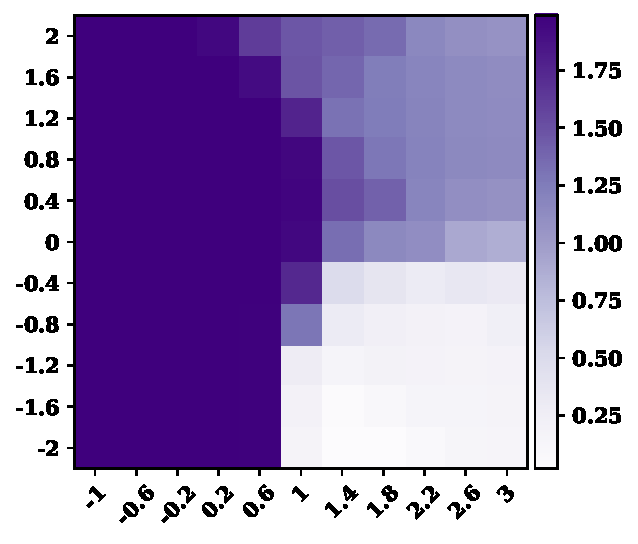
\includegraphics[width=.33\textwidth]{static/rounds_two_by_two_games_cooperation.pdf}
  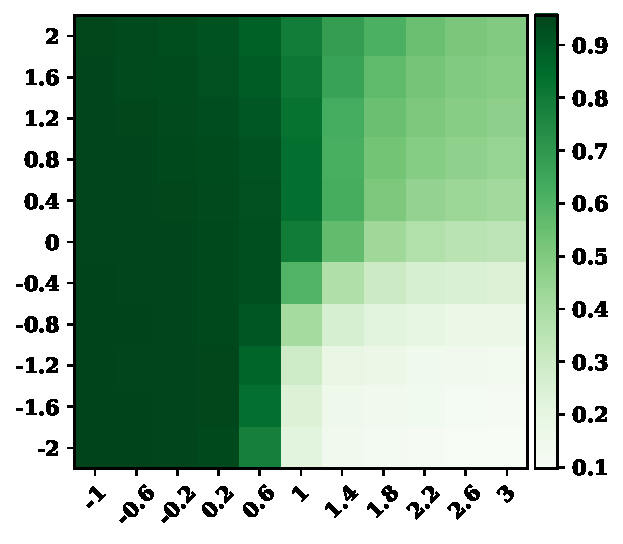
\includegraphics[width=.33\textwidth]{static/opponents_two_by_two_games_cooperation.pdf}
  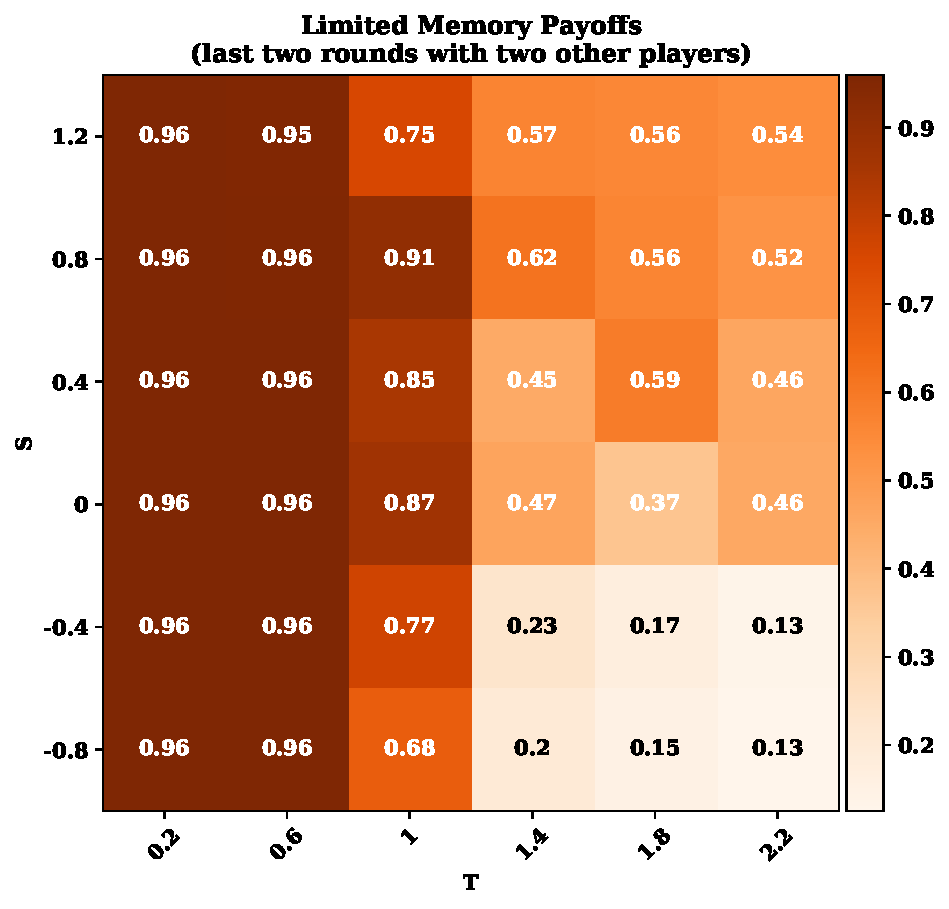
\includegraphics[width=.33\textwidth]{static/rounds_opponents_two_by_two_games_cooperation.pdf}
  \caption{\textbf{Cooperation rates over various social dilemmas for different
  limited memory payoffs.} ({\bf A}) If
  players update based on their last two rounds with another member of the population.
  ({\bf B}) If players update based on their last round with two other members of the population.
  ({\bf C}) If players update based on their last two rounds with two other members of the population.
  We vary the temptation
  payoff \(T \in \{0.2, 0.6, 1, 1.4, 1.8, 2.2\}\)
  across the \(x\) axis, and \(S \in \{1.2, 0.8, 0.4, 0, -0.4, -0.8\}\)
  across the \(y\) axis. Unless explicitly varied, the parameters of the simulation
  are $N\!=\!100$, $\beta\!=\!10$, $\delta\!=\!0.99$.}
  \label{fig:cooperation_rates_two_by_two_part_two}
\end{figure}


\section{Conclusions}\label{section:conclusions}

Evolutionary models have helped us understand the evolution of cooperation.
A behaviour so well observed in the world around us though Darwin spoke
about the survival of the fitness. Evolutionary

Much research in the past has been devoted to explore conditionally cooperative
strategies in pairwise interactions.

Previous models of direct reciprocity often feature a curious inconsistency.
When modeling how individuals make decisions in each round, these models assume
that players only remember the last round. However, when modeling how
individuals update their strategies over time, individuals are assumed to have
perfect memory. Here, we explore how robust our understanding of cooperation is
as models deviate from the perfect memory assumption. On the positive side, we
show that cooperation can even evolve when individuals only use a minimum of
information. On the negative side, the evolving cooperation rates are typically
lower than in the classical scenario.

In the case of the donation game we show that cooperation is overestimated.
Morover, we obsved that when the befenti and the srang f sleection increases this
difference becomes more obvuous, 


\appendix

\section{Model Setup}\label{appendix:methods}

Consider a population of \(N\) individuals where \(N\) is even. At any point in
time there are at most two different strategies in present in the population.
More specifically, a mutant strategy played by \(k\) individuals and a resident
strategy played by \(N - k\) individuals. We assume a pairwise process in which
strategies spread because they are imitated more often. Each step of the
evolutionary process consists of two stages; a game stage and an update stage.

In the game stage, each individual is randomly matched with some other
individual in the population. Their interaction lasts for a number of turns
which is not fixed but depends on the continuation probability \(\delta\). At
each turn the individuals choose between cooperation (\(C\)) and defection
(\(D\)). Thus, there are four possible outcomes in each turn \(CC, CD, DC\) and
\(DD\). If both players cooperate they receive the reward payoff \(R\), whereas
if both players defect they receive the punishment payoff \(P\). If one
cooperates but the other defects, the defector receives the temptation to
defect, \(T\), whereas the cooperator receives the sucker's payoff, \(S\).
Let $\mathcal{U}=\{R,S,T,P\}$ denote the set of feasible payoffs in each round,
and let $\mathbf{u}\!=\!(R,S,T,P)$ be the corresponding payoff vector.
The values of the payoffs are not only based on the prisoner's dilemma but all
the symmetric \(2 \times 2\) games, Table~\ref{table:social_dilemmas}.

A further assumption of our model is that individuals make use of reactive
strategies when they make decisions in each round. Reactive strategies are a set
of strategies that take into account only the previous action of the opponent.
A reactive strategy can be written explicitly as a vector,

\[s=(y, p, q)\]

where \(y\) is the probability that the strategy opens with a cooperation and
\(p, q\) are the probabilities that the strategy cooperates given that the
opponent cooperated and defected equivalently.

In the updating stage, two players are randomly drawn from the population, a
`learner' and a `role model'. The learner adopts the role model's strategy
based on the Fermi distribution function, %ToDo add reference

\begin{equation} \label{Eq:rho}
\rho(u_{L}, u_{RM}) = \frac{1}{1\!+\! \exp^{\!-\!\beta (u_{RM}\!-\!u_{L})}}.
\end{equation}

where $u_{L}\!\in\! \mathcal{U}$ is the learner's payoff, $u_{RM}\!\in\!
\mathcal{U}$ is the role model's payoff, and $\beta\!\ge\!0$ is the intensity of
selection.

We iterate this basic evolutionary step until either the mutant strategy goes
extinct, or until it fixes in the population and becomes the new resident
strategy. After either outcome, we set $k$ to $1$ and we introduce a new mutant
strategy which is uniformly chosen from all reactive strategies at random.
Instead of simulating each step of the evolutionary process, we estimate the
probability that a newly introduced mutant fixes~\cite{nowak2004emergence}. This
is defined as the fixation probability of the mutant, and the standard form is
the following,

\begin{equation}\label{eq:appendix_fixation_probability}
\varphi = \frac{1}{1+\sum\limits_{i=1}^{N-1}\prod\limits_k^i \frac{\lambda^-_k}{\lambda^+_k}},
\end{equation}

where \(\lambda^-_k, \lambda^+_k\) are the probabilities that the number of
mutants decreases and increases respectively.

This process of mutation and fixation/extinction is iterated many times. The
evolutionary process is summarized by
Algorithm~\ref{algorithm:pairwise_comparison}.

\begin{algorithm}[!htbp]
  \SetAlgoLined
   $N \leftarrow$ population size\;
   $k \leftarrow 1$\;
   resident $\leftarrow (0, 0, 0)$\;
   \While{step $<$ maximum number of steps}{
    mutant $\leftarrow$ random: $\{\emptyset \}\ \rightarrow R^3$\;
    fixation probability $\leftarrow \varphi $\;
    \If{$\varphi >$ random: $i \rightarrow [0, 1]$}{
      resident $\leftarrow$ mutant;
     }}
     \caption{Evolutionary process}\label{algorithm:pairwise_comparison}
\end{algorithm}

The aim of this work is to explore the effect of updating memory on the
cooperation rate of the evolved population. For this reason we consider two
different approaches when estimating the payoffs at the updating stage. The two
approaches we consider are those of (i) the expected and (ii) the limited memory
payoffs.

\subsection*{Expected Payoffs}

The expected payoffs are the conventional payoffs used in the updating
stage~\cite{imhof2010stochastic}. They are defined as the mean payoff of an
individual in a well-mixed population that engages in repeated games with all
other population members.

We first define the payoff of two reactive strategies at the game stage. Assume
two reactive strategies $s_1\!=\!(y_1, p_1, q_1$) and $s_2\!=\!(y_2,p_2,q_2)$.
It is not necessary to simulate the play move by move, instead the play between
the two strategies is defined a Markov matrix \(M\),

\begin{equation}\label{eq:transition_matrix}
  M = \left[\begin{matrix} p_{1} p_{2} & p_{1} \left(1 - p_{2}\right) & p_{2} \left(1 - p_{1}\right) & \left(1 - p_{1}\right) \left(1 - p_{2}\right)\\
    p_{2} q_{1} & q_{1} \left(1 - p_{2}\right) & p_{2} \left(1 - q_{1}\right) & \left(1 - p_{2}\right) \left(1 - q_{1}\right)\\
    p_{1} q_{2} & p_{1} \left(1 - q_{2}\right) & q_{2} \left(1 - p_{1}\right) & \left(1 - p_{1}\right) \left(1 - q_{2}\right)\\
    q_{1} q_{2} & q_{1} \left(1 - q_{2}\right) & q_{2} \left(1 - q_{1}\right) & \left(1 - q_{1}\right) \left(1 - q_{2}\right)\end{matrix}\right].
\end{equation}

whose stationary vector \(\mathbf{v}\), combined with the payoff \(u\), yields
the game stage outcome for each strategy,
\(\langle\mathbf{v}(s_1,s_2),\mathbf{u}\rangle\)~\cite{Hauert1997}.


In the updating stage the learner adopts the strategy of the role model based on
their updating payoffs. Given that there are only two different types in the
population at each time step we only need to define the expected payoff for a
resident (\(\pi_R\)) and for a mutant (\(\pi_M\)). Assume the resident strategy
\(s_R = (y_R, p_R, q_R)\) and the mutant strategy \(s_M = (y_M, p_M, q_M)\), the
expected payoffs are give by,

\begin{equation} \label{Eq:ExpPay}
  \begin{array}{lcrcr}
  \displaystyle \pi_R	&=	&\displaystyle \frac{N\!-\!k\!-\!1}{N-1}\cdot \langle\mathbf{v}(s_R,s_R),\mathbf{u}\rangle	&+	&\displaystyle\frac{k}{N-1}\cdot \langle\mathbf{v}(s_R,s_M),\mathbf{u}\rangle,\\[0.5cm]
  \displaystyle \pi_M	&=	&\displaystyle\frac{N-k}{N-1}\cdot \langle\mathbf{v}(s_M,s_R),\mathbf{u}\rangle&+	&\displaystyle\frac{k-1}{N-1}\cdot \langle\mathbf{v}(s_M,s_M),\mathbf{u}\rangle.\\
  \end{array}
\end{equation}

The number of mutant in the population increase if a learner resident adopts the
strategy of a mutant role model, and decreases if a mutant leaner adopts the
strategy of a resident. The probabilities that the number of mutants decreases
and increases, \(\lambda^-_k\) and \(\lambda^+_k\), are now explicitly defined
as,

\begin{align*} 
  \lambda^-_k &\!=\!\rho(\pi_R, \pi_M) \\
  \lambda^+_k &\!=\!\rho(\pi_M, \pi_R).
\end{align*}

\subsection*{Limited memory payoffs}

Initially, we discuss the case of the last round updating payoff. At the stage
game we define the payoff of a reactive strategy in the last round,
Proposition~\ref{proposition:last_round}.


\begin{Prop}\label{proposition:last_round}
    Consider a repeated prisoner's dilemma, with
    continuation probability $\delta$, between players with reactive strategies
    $s_1\!=\!(y_1, p_1, q_1$)  and $s_2\!=\!(y_2,p_2,q_2)$ respectively. Then the
    probability that the $s_1$ player receives the payoff $u\!\in\! \mathcal{U}$ in
    the very last round of the game is given by $v_{u}(s_1,s_2)$, as given by
    Equation~(\ref{Eq:LastRound}).

    \begin{equation} \label{Eq:LastRound}
      \setlength{\arraycolsep}{1pt}
      \begin{array}{rcl}
    
      v_{R}(s_1,s_2) &= &\displaystyle (1\!-\!\delta)\frac{y_1y_2}{1\!-\!\delta^2 r_1 r_2}+\delta \frac{\Big(q_1+r_1\big((1\!-\!\delta)y_2+\delta q_2\big)\Big) \Big(q_2+r_2\big((1\!-\!\delta)y_1+\delta q_1\big)\Big)}
      {\displaystyle(1\!-\!\delta r_1r_2)(1\!-\!\delta^2 r_1 r_2)} \times R,\\[1cm]
    
      v_{S}(s_1,s_2) &= &\displaystyle (1\!-\!\delta)\frac{y_1\bar{y}_2}{1\!-\!\delta^2 r_1 r_2}+\delta \frac{\Big(q_1+r_1\big((1\!-\!\delta)y_2+\delta q_2\big)\Big) \Big(\bar{q}_2+\bar{r}_2\big((1\!-\!\delta)y_1+\delta p_1\big)\Big)}
      {\displaystyle(1\!-\!\delta r_1r_2)(1\!-\!\delta^2 r_1 r_2)} \times S,\\[1cm]
    
      v_{T}(s_1,s_2) &= &\displaystyle (1\!-\!\delta)\frac{\bar{y}_1y_2}{1\!-\!\delta^2 r_1 r_2}+\delta \frac{\Big(\bar{q}_1+\bar{r}_1\big((1\!-\!\delta)y_2+\delta p_2\big)\Big) \Big(q_2+r_2\big((1\!-\!\delta)y_1+\delta q_1\big)\Big)}
      {\displaystyle(1\!-\!\delta r_1r_2)(1\!-\!\delta^2 r_1 r_2)} \times T,\\[1cm]
    
      v_{P}(s_1,s_2) &= &\displaystyle (1\!-\!\delta)\frac{\bar{y}_1\bar{y}_2}{1\!-\!\delta^2 r_1 r_2}+\delta \frac{\Big(\bar{q}_1+\bar{r}_1\big((1\!-\!\delta)y_2+\delta p_2\big)\Big) \Big(\bar{q}_2+\bar{r}_2\big((1\!-\!\delta)y_1+\delta p_1\big)\Big)}
      {\displaystyle(1\!-\!\delta r_1r_2)(1\!-\!\delta^2 r_1 r_2)} \times P.
      \end{array}
    \end{equation}

In these expressions, we have used the notation $r_i:=p_i\!-\!q_i$,
$\bar{y}_i\!=\!1\!-\!y_i$, $\bar{q}_i:=1\!-\!q_i$, and
$\bar{r}_i:=\bar{p}_i\!-\!\bar{q}_i=-r_i$ for $i\!\in\!\{1,2\}$.
\end{Prop}

\begin{proof}
Given a play between two reactive strategies with continuation probability
$\delta$. The outcome at turn \(t\) is given by,

\begin{equation}\label{eq:}
  (1 - \delta) \mathbf{v_0} \sum \delta^{t} M^{(t)},
\end{equation}

where $\mathbf{v_0}$ denotes the expected distribution of the four outcomes in
the very first round, and \(1- \delta\) the probability that the game ends.
It can be shown that,

\begin{align*}
  (1 - \delta) \mathbf{v_0} \sum \delta^{t} M^{(t)} & = (1 - \delta)(\mathbf{v_0} + \delta \mathbf{v_0} M + \delta^{2}\mathbf{v_0} M ^{2} + \dots )\\ 
   & = (1 - \delta)\mathbf{v_0} (1 + \delta M + \delta^{2}M ^{2} + \dots ) \text{ using standard formula for geometric series}\\ 
   & = (1 - \delta)\mathbf{v_0}(I_4 - \delta M)^{-1}
\end{align*}

where \((1 - \delta)\mathbf{v_0}(I_4 - \delta M)^{-1}\) is vector \(\in R^{4}\)
and it the probabilities for being in any of the outcomes \(CC, CD, DC, DD\) in
the last round. Combining this with the payoff vector \(u\) and some algebraic
manipulation we derive to the Equation~\ref{Eq:LastRound}.
\end{proof}

In the updating stage we select a mutant and resident to be either the role
model or the learner. Given that they can interact with only one other member of
the population, they can interact either with each other or either can interact
with another resident or with another mutant. Thus, in each updating stage there
are five possible combinations of pairs. These are illustrated by
Figure~\ref{fig:single_pairs}.

\begin{figure}[!htbp]
  \centering
  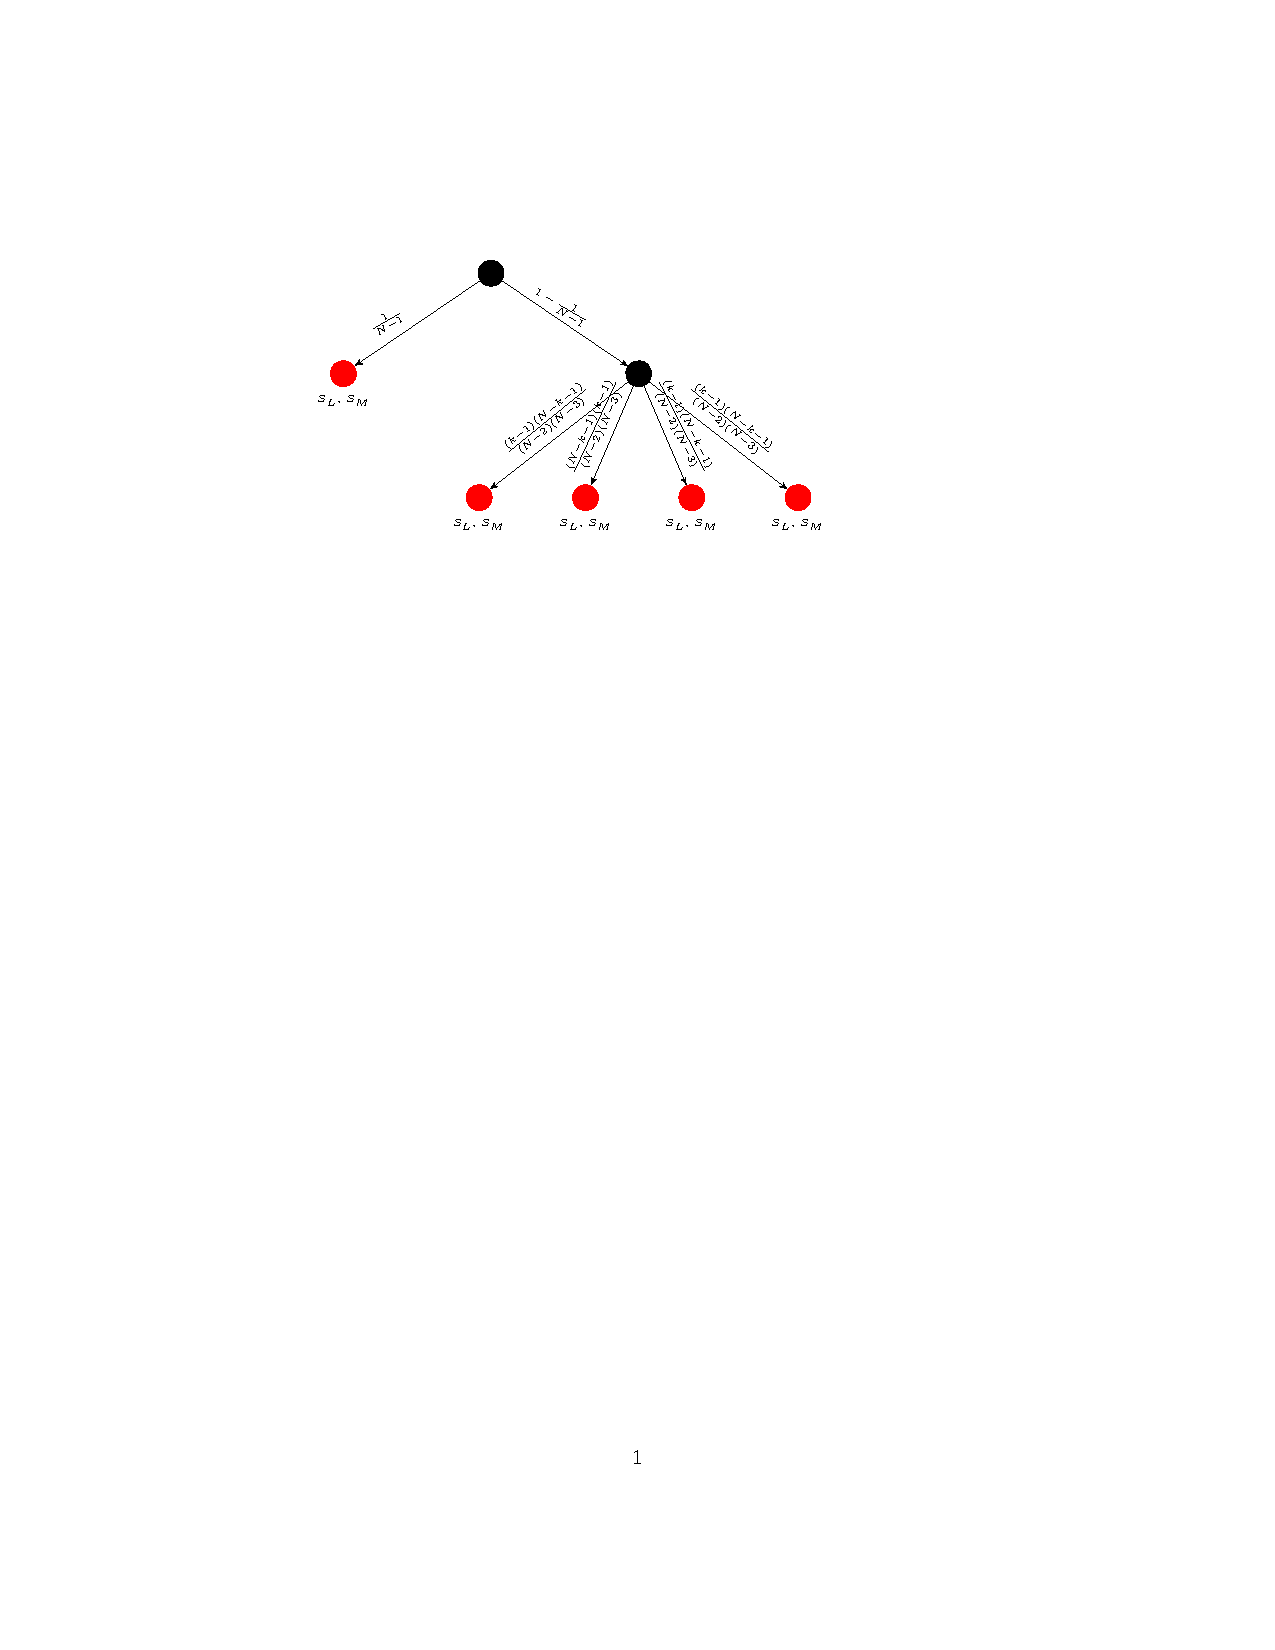
\includegraphics[width=.65\textwidth]{static/last_rounds_matches.tex}
  \caption{\textbf{Possible pairings combination in the updating stage, given
  that individuals interact with only one other member in the population.}}
  \label{fig:single_pairs}
\end{figure}

The probability that the respective payoffs of the players
are given by $u_1$ and $u_2$ can be calculated as

\begin{equation}\label{eq:Chi}
\setlength{\arraycolsep}{1pt}
\begin{array}{llrl}
x(u_1,u_2)	 &=&\displaystyle \frac{1}{N\!-\!1}\cdot  &v_{u_1}(S_1,S_2)\cdot 1_{(u_1,u_2)\in \mathcal{U}^2_F}\\[0.5cm]
&+	
&\displaystyle \left(1\!-\!\frac{1}{N\!-\!1}\right)  
&\left[ \frac{k\!-\!1}{N\!-\!2}\frac{k\!-\!2}{N\!-\!3} v_{u_1}(S_1,S_2) v_{u_2}(S_2,S_2) + 
 \frac{k\!-\!1}{N\!-\!2}\frac{N\!-\!k\!-\!1}{N\!-\!3} v_{u_1}(S_1,S_2) v_{u_2}(S_2,S_1)\right.\\[0.5cm]
&&&\left. +\frac{N\!-\!k\!-\!1}{N\!-\!2}\frac{k\!-\!1}{N\!-\!3} v_{u_1}(S_1,S_1) v_{u_2}(S_2,S_2) + 
 \frac{N\!-\!k\!-\!1}{N\!-\!2}\frac{N\!-\!k\!-\!2}{N\!-\!3} v_{u_1}(S_1,S_1) v_{u_2}(S_2,S_1)\right].
\end{array}
\end{equation}

The first term on the right side corresponds to the case that the learner and
the role model happened to be matched during the game stage, which happens with
probability $1/(N\!-\!1)$.In that case, we note that only those payoff pairs
can occur that are feasible in a direct interaction, $\splitatcommas{(u_1,u_2)\in
\mathcal{U}^2_F:=\big\{ (R,R), (S,T), (T,S), (P,P) \big\}}$, as represented by
the respective indicator function. Otherwise, if the learner and the role model
did not interact directly, we need to distinguish four different cases,
depending on whether the learner was matched with a resident or a mutant, and
depending on whether the role model was matched with a resident or a mutant.

Given that $N\!-\!k$ players use the resident strategy $s_{R}\!=\!(y_{R},p_{R},q_{R})$
and that the remaining $k$ players use the mutant strategy
$S_{M}\!=\!(y_{M},p_{M},q_{M})$, the probability that the number of mutants increases by
one in one step of the evolutionary process can be written as

\begin{align}
\lambda^+_k=\frac{N\!-\!k}{N}\cdot \frac{k}{N}\cdot \sum_{u_{R},u_{M}\in\mathcal{U}} x(u_{R},u_{M})\cdot \rho(u_{R},u_{M}), \\
\lambda^-_k=\frac{N\!-\!k}{N}\cdot \frac{k}{N}\cdot \sum_{u_{R},u_{M}\in\mathcal{U}} x(u_{R},u_{M})\cdot \rho(u_{M},u_{R}).
\end{align}

In this expression, $(N\!-\!k)/N$ is the probability that the randomly chosen
learner is a resident, and $k/N$ is the probability that the role model is a
mutant. The sum corresponds to the total probability that the learner adopts the
role model's strategy over all possible payoffs $u_1$ and $u_2$ that the two
player may have received in their respective last rounds. We use $x(u_1,u_2)$ to
denote the probability that the randomly chosen resident obtained a payoff of
$u_1$ in the last round of his respective game, and that the mutant obtained a
payoff of $u_2$.

This framework can be extended to consider the case of where the payoffs
correspond to the last \(n\) rounds payoff an individual achieved after
interacting with \(m\) other individuals. For the case \(n=2\) the payoffs
at the game stage are,

\begin{Prop}\label{proposition:last_two_rounds}
Assume a play between the reactive strategies \(s_1\) and \(s_2\) with a
continuation probability \(\delta\). Then the probability of being in any of the
sixteen outcomes \(\splitatcommas{RR, RS, RT, RP, SR, SS, ST, SP, TR, TS, TT, TP, PR, PS, PT, PP}\)
on the last two rounds are given by,

\begin{equation}
  \mathbf{v_{a_1, a_2}} = (1 - \delta) m_{a_1, a_2} \delta^2 \left[\mathbf{v_0}(I_4 - \delta M)^{-1}\right]_{a_1, a_2}, \quad \text{ for } m_{a_1, a_2} \in M \ \& \ a_1, a_2 \in \{R, S, T, P\}
\end{equation}

\end{Prop}

Equation~\ref{eq:Chi} can also be extended to include interactions with two
other individuals. The possible pairings are illustrated by
Figure~\ref{fig:pissible_two_pairs}.

\begin{figure}[!htbp]
  \centering
  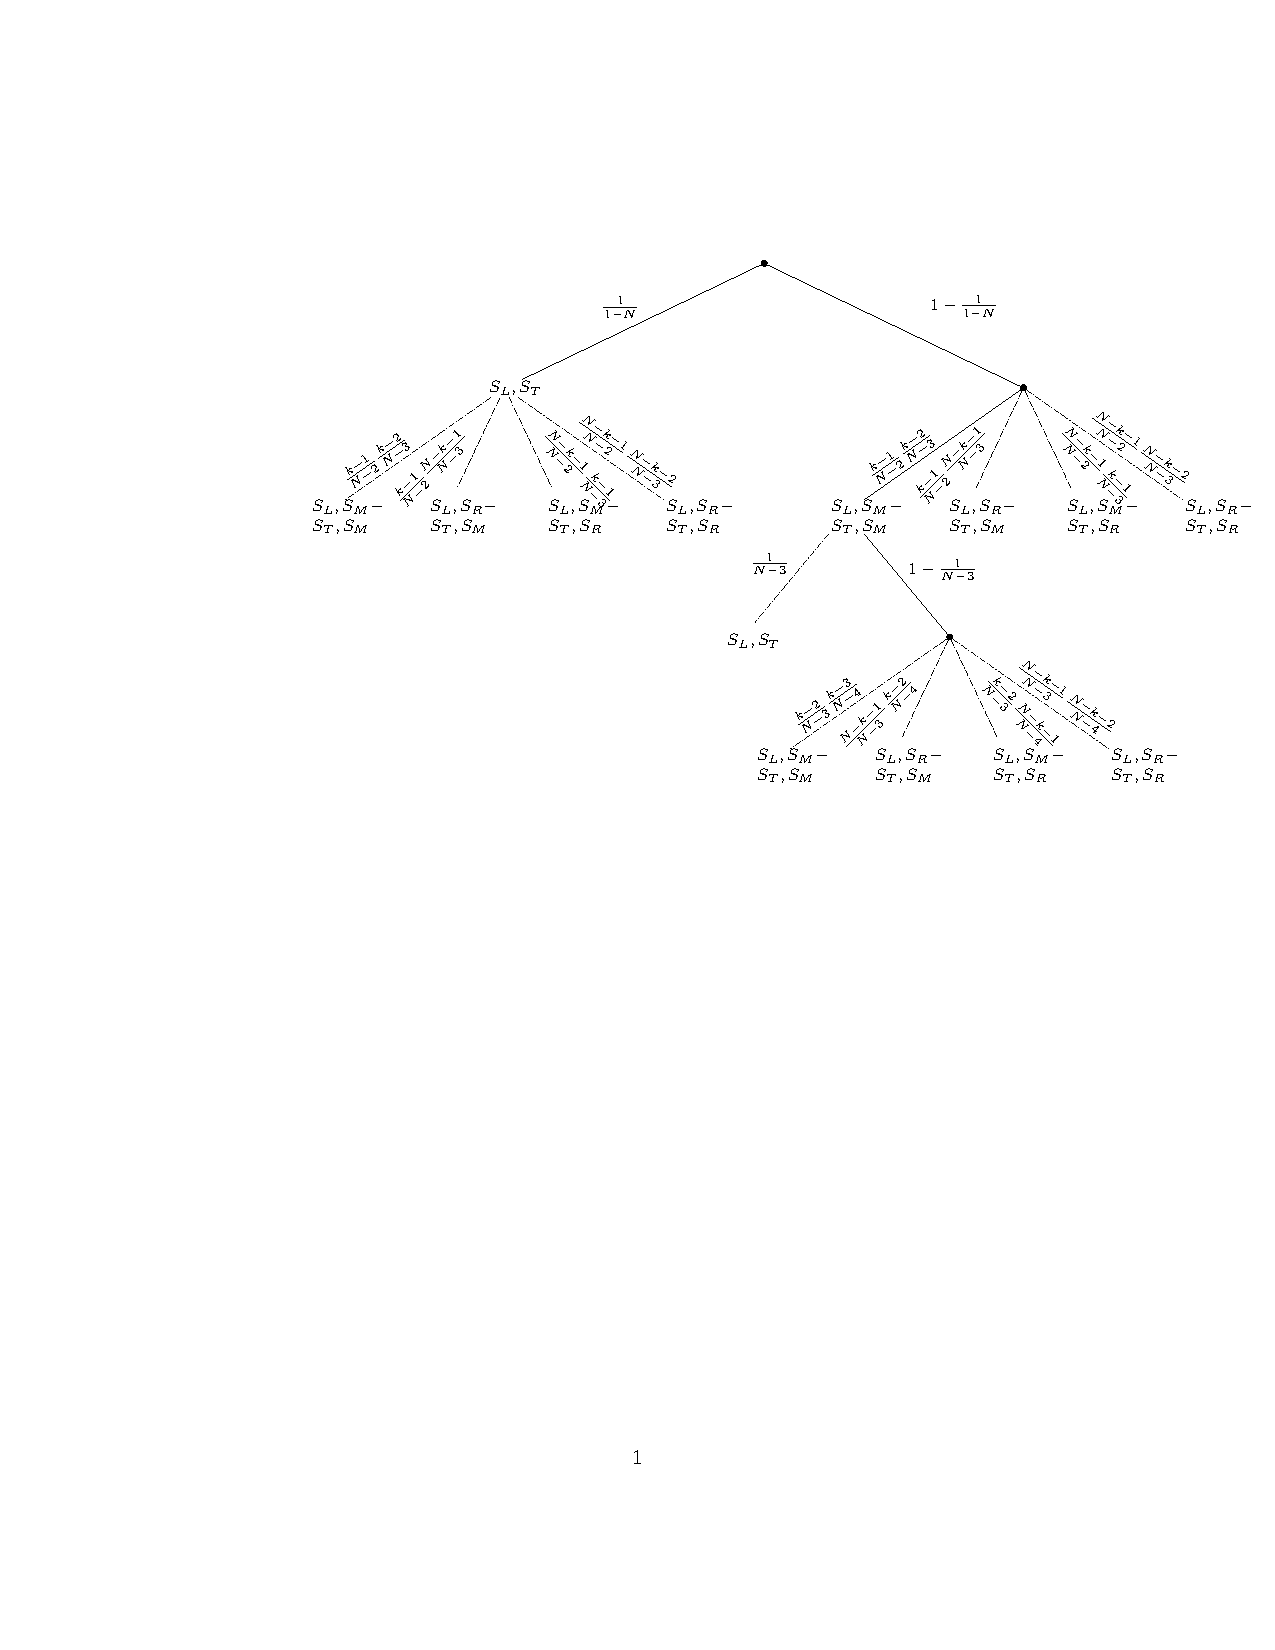
\includegraphics[width=.65\textwidth]{static/tree.tex}
  \caption{\textbf{Possible pairings combination in the updating stage, given
  that individuals interact with two other members in the population.}}
  \label{fig:pissible_two_pairs}
\end{figure}

Simulating the evolutionary process for longer memory quickly becomes
computationally untractable. Our methodology could be extended to include more
turns and more interactions. However, for the purpose of this work we explore
the cases only up to two turns and two interactions.


\section{Evolutionary dynamics under limited memory payoffs for various social dilemmas}\label{appendix:further_simulation_results}

\begin{figure}[!htbp]
  \centering
  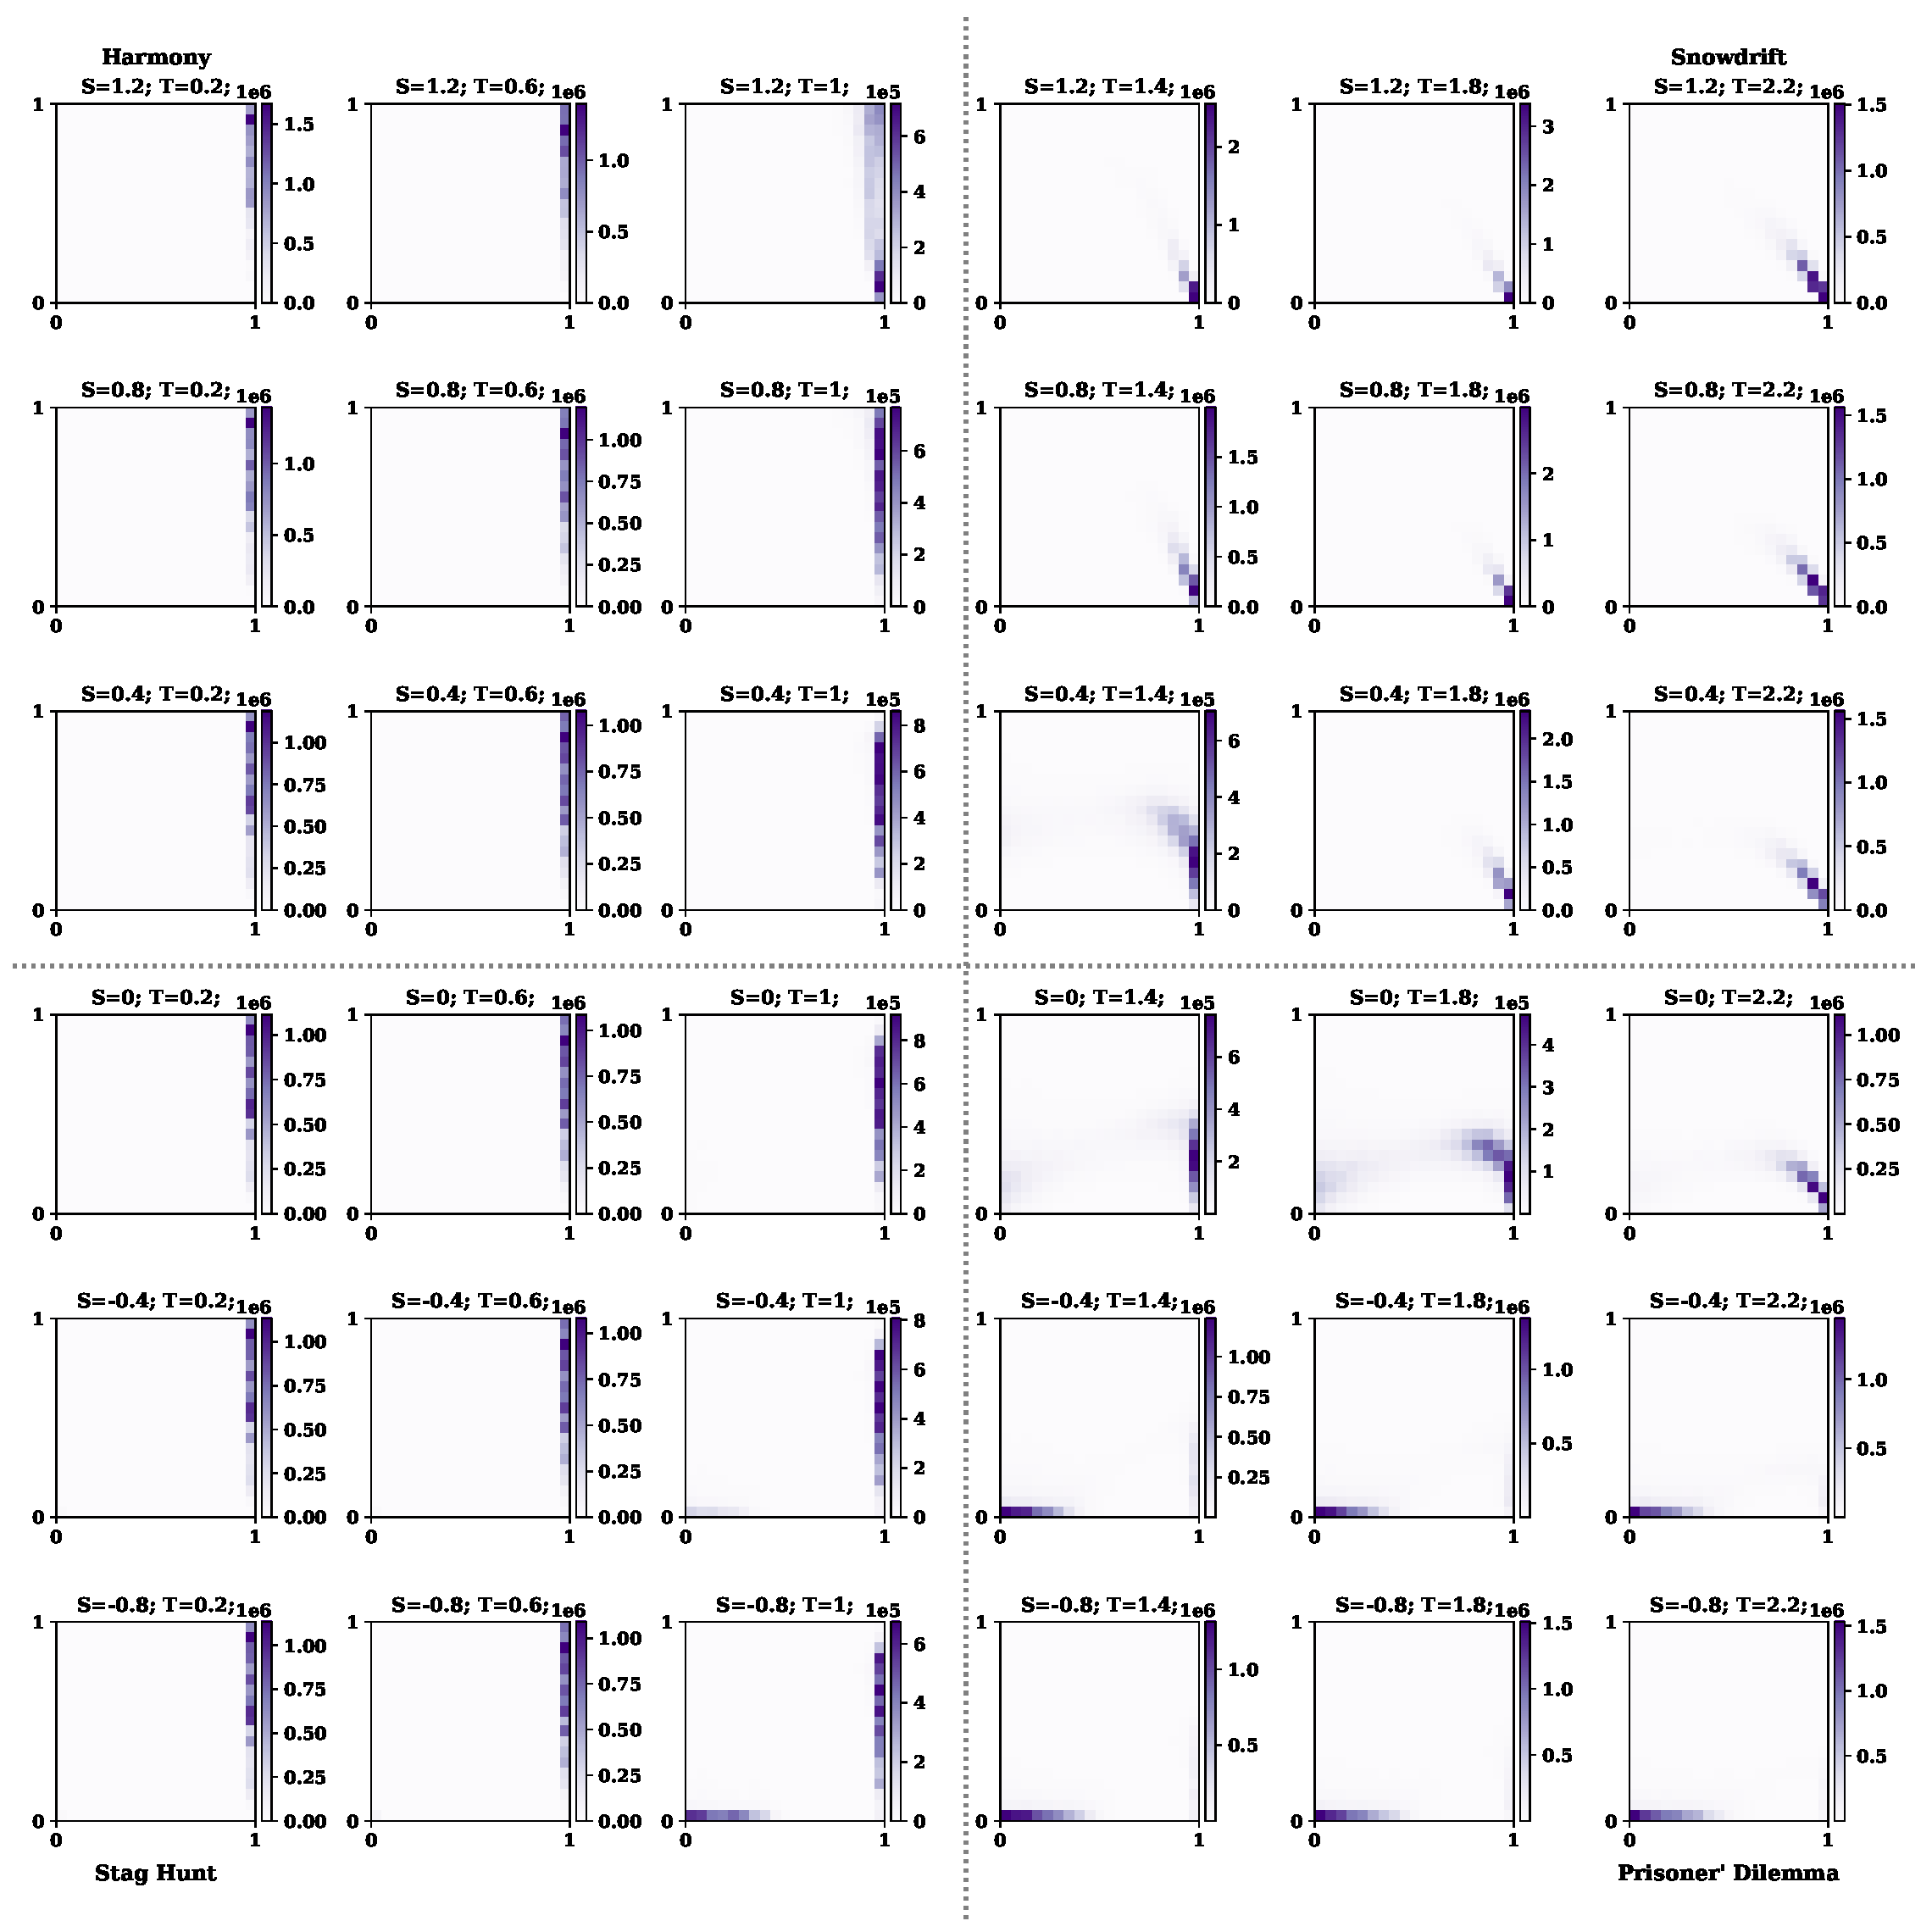
\includegraphics[width=\textwidth]{static/rounds_two_by_two_games.pdf}
  \caption{{\bf Evolutionary dynamics under last two rounds payoffs for various social dilemmas.} 
  We have run several simulations of the evolutionary process described in
  section~\ref{section:model} for $T\!=\!10^7$ time steps. The graphs show how
  often the resident population chooses each combination ($p,q$) of conditional
  cooperation probabilities in the subsequent rounds. We vary the temptation
  payoff \(T \in \{-1, -0.6, -0.2,  0.2, 0.6, 1, 1.4, 1.8, 2.2, 2.6, 3\}\)
  across the \(x\) axis, and  \(S \in \{2, 1.6, 1.2, 0.8, 0.4, 0, -0.4, -0.8,
  -1.2, -1.6, -2\}\) across the \(y\) axis. Parameters: $N\!=\!100$,
  $\beta\!=\!10$, $\delta\!=\!0.999$.}
  \label{fig:last_two_rounds_two_by_two}
\end{figure}

\begin{figure}[!htbp]
  \centering
  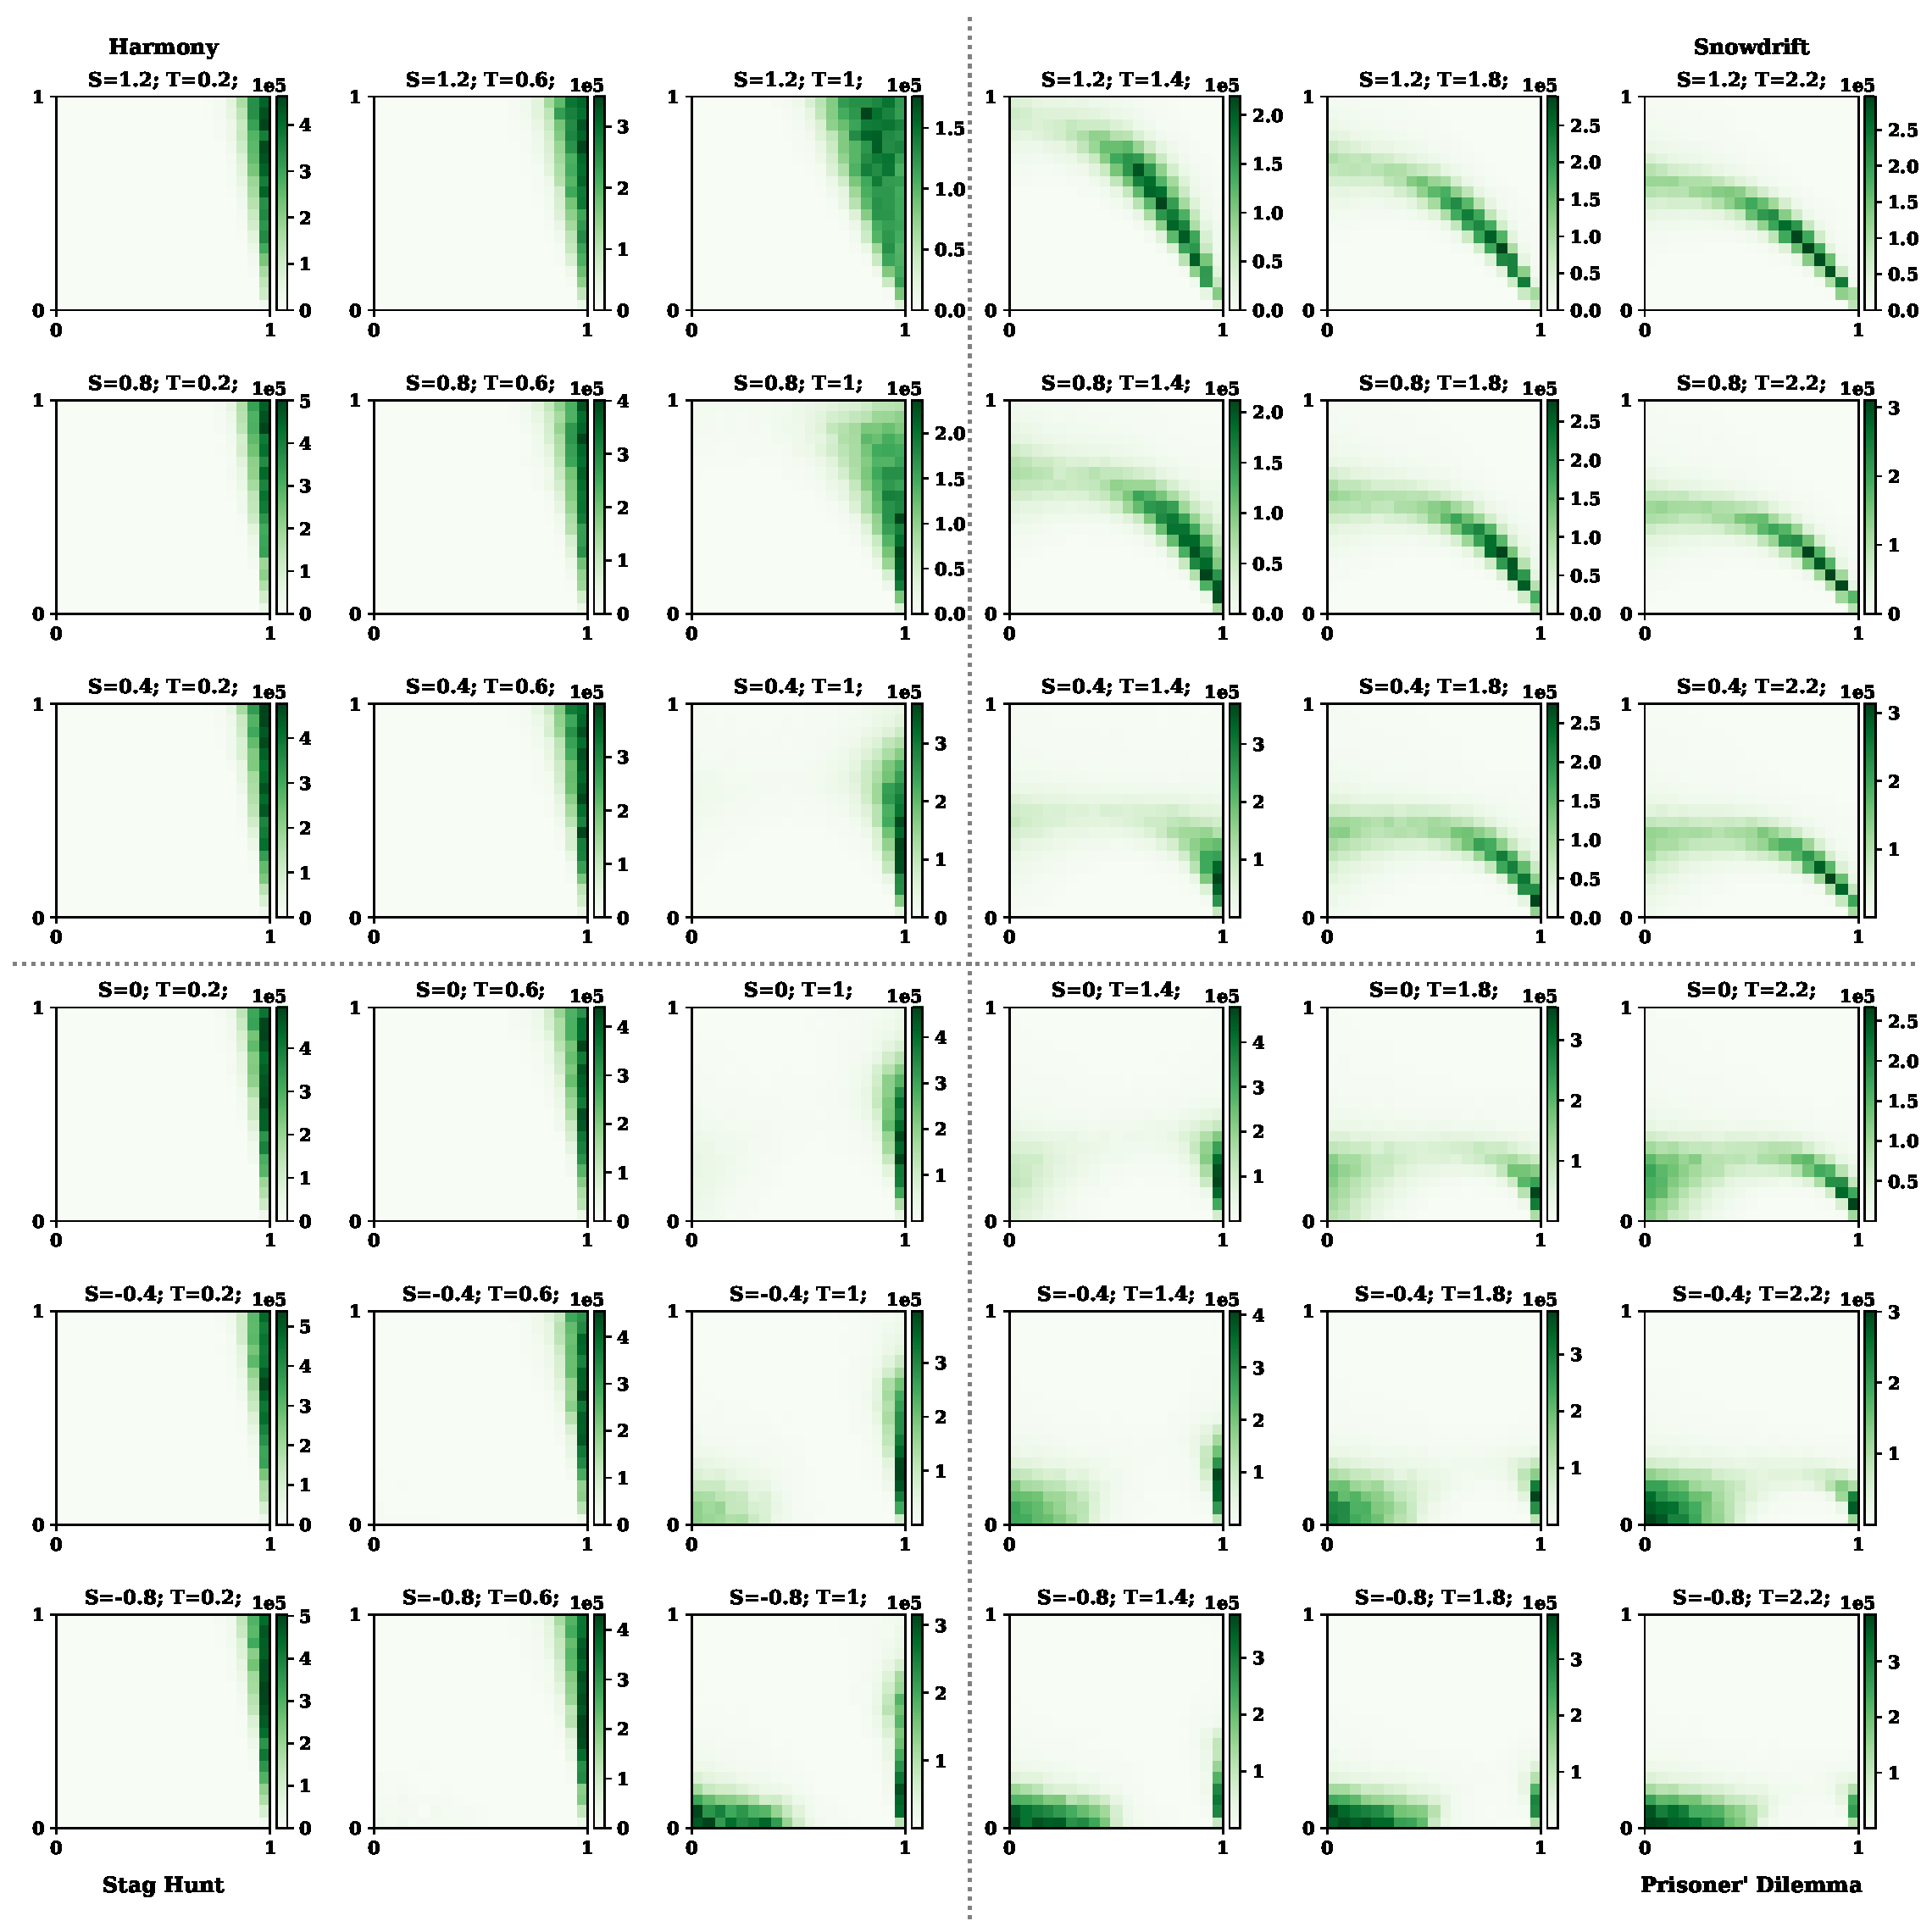
\includegraphics[width=\textwidth]{static/opponents_two_by_two_games.pdf}
  \caption{{\bf Evolutionary dynamics under last round payoffs with two members of the population for various social dilemmas.} 
  We have run several simulations of the evolutionary process described in
  section~\ref{section:model} for $T\!=\!10^7$ time steps. The graphs show how
  often the resident population chooses each combination ($p,q$) of conditional
  cooperation probabilities in the subsequent rounds. We vary the temptation
  payoff \(T \in \{-1, -0.6, -0.2,  0.2, 0.6, 1, 1.4, 1.8, 2.2, 2.6, 3\}\)
  across the \(x\) axis, and  \(S \in \{2, 1.6, 1.2, 0.8, 0.4, 0, -0.4, -0.8,
  -1.2, -1.6, -2\}\) across the \(y\) axis. Parameters: $N\!=\!100$,
  $\beta\!=\!10$, $\delta\!=\!0.999$.}
  \label{fig:last_two_opponents_two_by_two}
\end{figure}

\begin{figure}[!htbp]
  \centering
  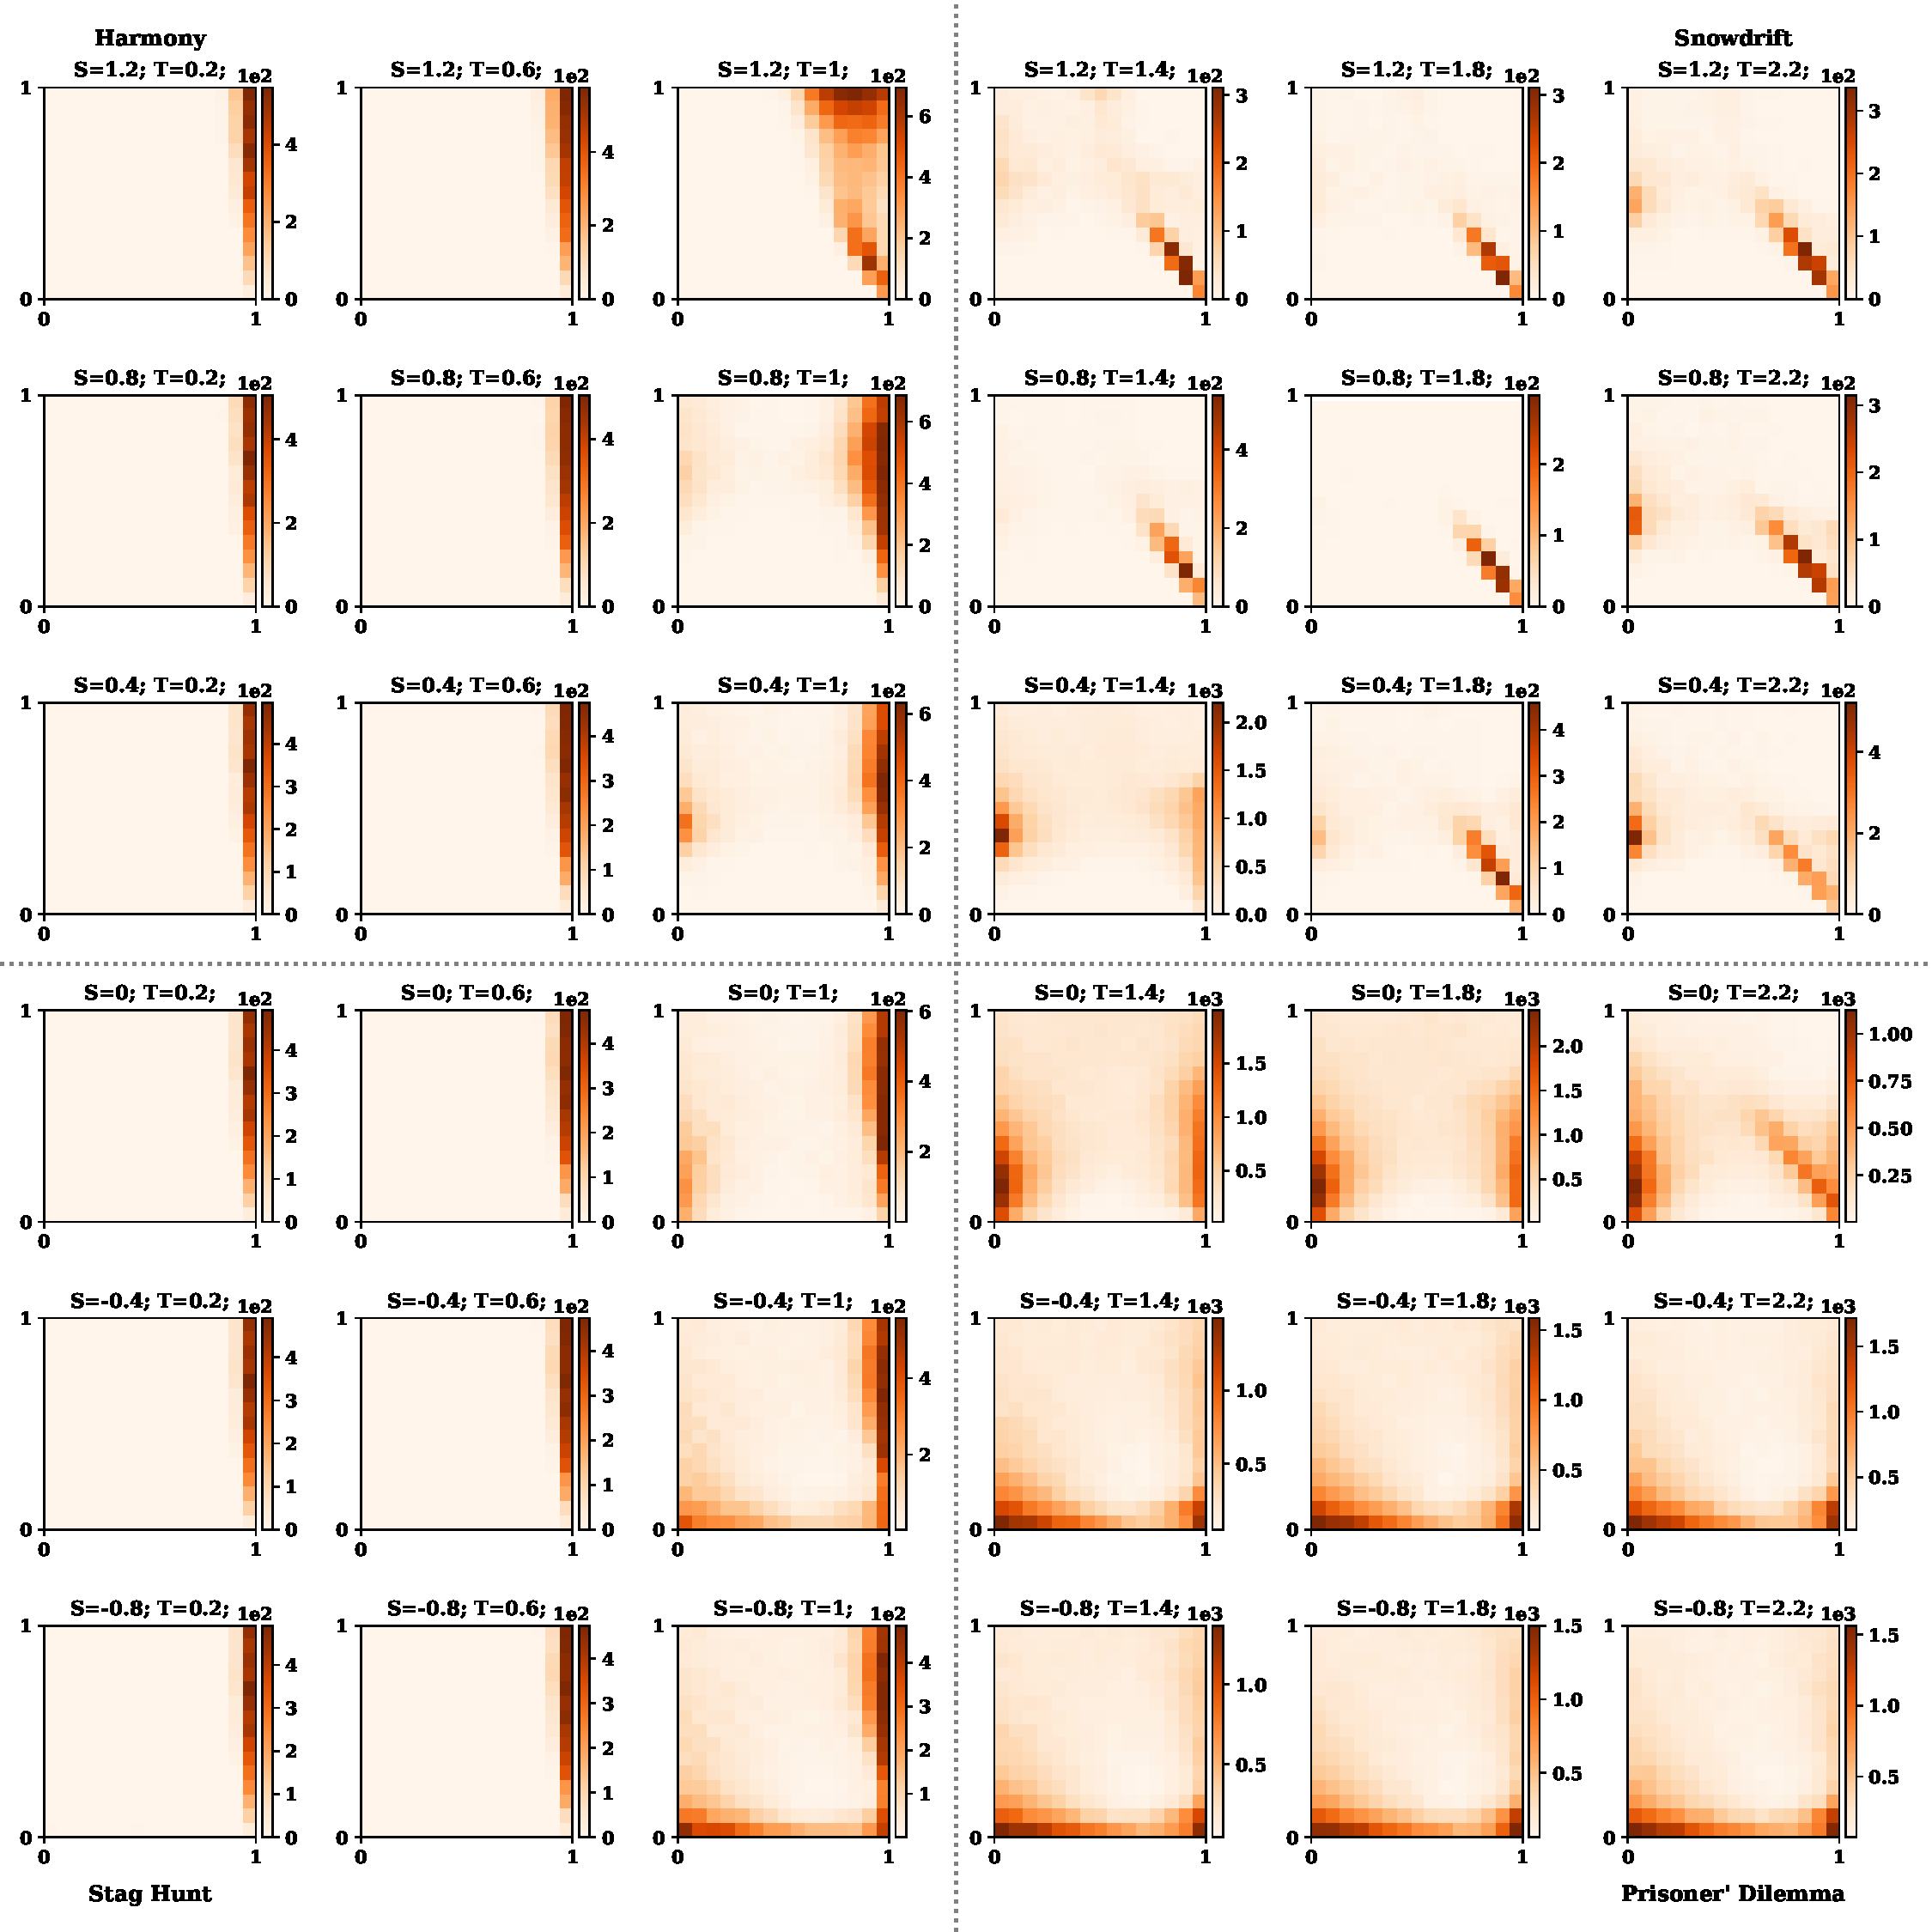
\includegraphics[width=\textwidth]{static/merged_plot_rounds_opponents_two.pdf}
  \caption{{\bf Evolutionary dynamics under last two rounds payoffs with two members of the population for various social dilemmas.} 
  We have run several simulations of the evolutionary process described in
  section~\ref{section:model} for $T\!=\!10^7$ time steps. The graphs show how
  often the resident population chooses each combination ($p,q$) of conditional
  cooperation probabilities in the subsequent rounds. We vary the temptation
  payoff \(T \in \{-1, -0.6, -0.2,  0.2, 0.6, 1, 1.4, 1.8, 2.2, 2.6, 3\}\)
  across the \(x\) axis, and  \(S \in \{2, 1.6, 1.2, 0.8, 0.4, 0, -0.4, -0.8,
  -1.2, -1.6, -2\}\) across the \(y\) axis. Parameters: $N\!=\!100$,
  $\beta\!=\!10$, $\delta\!=\!0.999$.}
  \label{fig:last_two_rounds_two_opponents}
\end{figure}

\begin{figure}[!htbp]
  \centering
  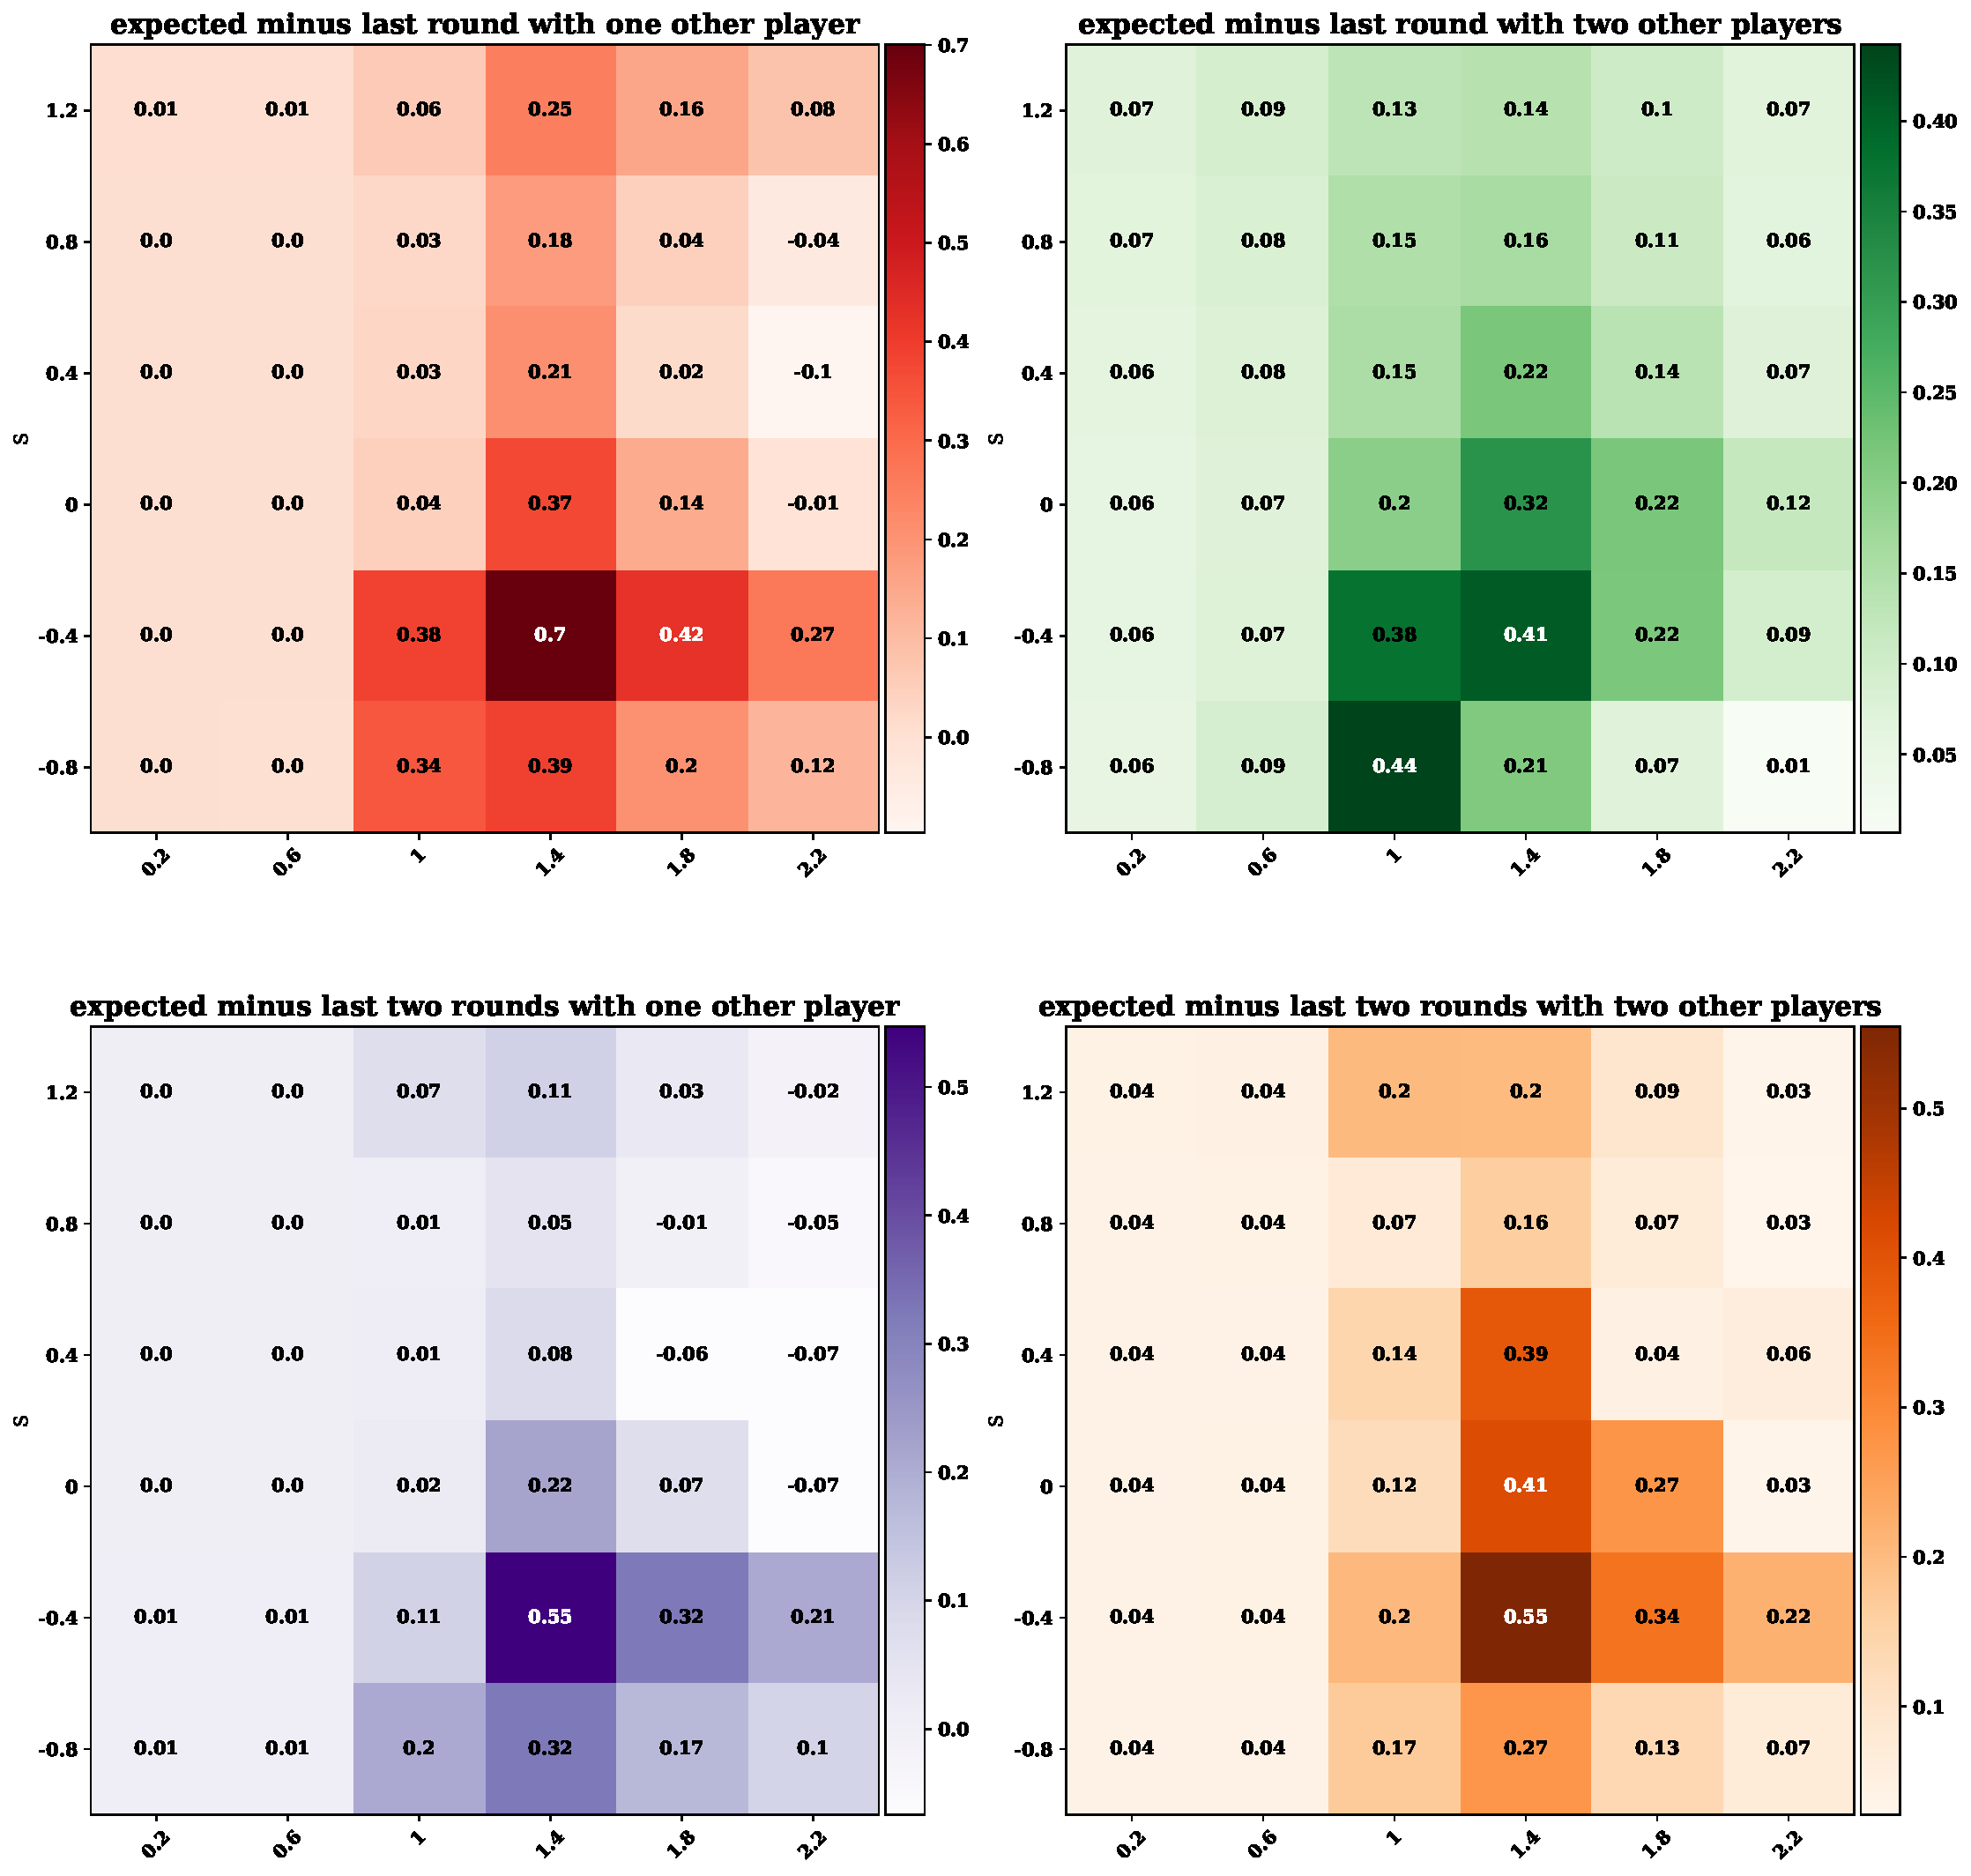
\includegraphics[width=\textwidth]{static/difference_in_cooperation.pdf}
  \caption{{\bf The difference in cooperate rates for each method compared to the
  expected payoffs.}}
  % \label{fig:last_two_rounds_two_opponents}
\end{figure}

\bibliographystyle{unsrt}
\bibliography{bibliography.bib}



\end{document}
